\documentclass[11pt]{article}

\usepackage{geometry}
\usepackage[T1]{fontenc}
\usepackage[utf8]{inputenc}
\usepackage{lmodern}
\usepackage{amsmath,amssymb,amsthm,amsfonts}
\usepackage{booktabs}
\usepackage{graphicx}
\usepackage{siunitx}
\usepackage[numbers]{natbib}
\usepackage{hyperref}
\usepackage[nameinlink,noabbrev]{cleveref}
\usepackage{setspace}
\usepackage{subcaption}
\usepackage{placeins}
\geometry{a4paper,margin=2.5cm}
\usepackage{changepage}
\usepackage[normalem]{ulem}
\usepackage{authblk}
\usepackage{array}
\usepackage[table]{xcolor}
\usepackage{tabularx}
\usepackage{tikz}
\usetikzlibrary{arrows.meta,positioning,plotmarks}
\InputIfFileExists{generated/spoofing_empirical_macros.tex}{}{}

\onehalfspacing
\hypersetup{
    colorlinks=true,
    linkcolor=blue,
    citecolor=blue,
    urlcolor=blue,
    pdftitle={Detecting Spoofing in Electronic Markets},
    pdfauthor={Daniele Maria Di Nosse, Francesco Gigante, Antonio Russo, Fabrizio Lillo}
}


\title{An Auditable Market-Microstructure Framework for Spoofing-Compatible Sequence Detection}
\author[1]{Daniele Maria Di Nosse\textsuperscript{\dag}}
\author[2]{Francesco Gigante}
\author[2]{Antonio Russo}
\author[1]{Fabrizio Lillo}

\affil[1]{Scuola Normale Superiore, Pisa, Italy}
\affil[2]{Consob, Rome, Italy}
\date{\today}

\begin{document}

\maketitle
\begin{center}
  \footnotesize
  \dag Corresponding author. Email: \texttt{daniele.dinosse@sns.it}
\end{center}

\begin{abstract}
We develop an auditable microstructure framework for screening order-book sequences that are compatible with spoofing.
Legitimate liquidity provision remains an explicit alternative explanation. The framework reconstructs the visible limit
order book, consolidates related passive child fills into execution clusters, and links each cluster to same-client orders
posted on the opposite side during the preceding $90$ seconds and withdrawn within $2$ seconds after the cluster. An
empirical top-$10$ depth kernel weights visible liquidity by book rank. We apply the framework to three Italian equity
samples and report mechanical withdrawal and price-response diagnostics. The resulting conjunction supports reproducible
surveillance triage. It does not constitute a statistical test, identify manipulative intent, estimate causal effects, or
measure the prevalence of spoofing.
\end{abstract}

\paragraph{Keywords.}
Spoofing detection; market manipulation; limit order book; high-frequency trading; anomaly detection; market maker; market microstructure

\section{Introduction}
\label{sec:introduction}
Electronic continuous double auctions organize price discovery through a limit order book (LOB). The LOB records the
visible bid and ask orders submitted by market participants and changes whenever an order is entered, amended, executed,
or cancelled. Algorithmic and high-frequency trading have increased the speed of these updates and can improve short-term
liquidity. The same speed also allows a participant to create and remove large displayed positions before other traders
can assess the full sequence.

Spoofing exploits this sequencing problem. In the stylized mechanism, a participant submits a large order on one side of
the LOB without intending to execute it. The displayed quantity can create a misleading signal of supply or demand and
can alter order-book imbalance or microprice indicators. Other participants may respond by changing their quotes or
submitting aggressive orders. The participant can then execute a smaller order on the opposite side at a more favorable
price and withdraw the large displayed order. The Market Abuse Regulation (MAR) prohibits orders and behavior that create
false or misleading signals about the supply of, demand for, or price of a financial instrument \cite{EU5962014}.

The observable actions in this mechanism are not unique to spoofing. Liquidity providers also submit, amend, and cancel
orders at high frequency, and they may have high order-to-trade ratios. They remove quotes to update prices,
control inventory, or limit adverse selection. Static size thresholds, cancellation ratios, and volumetric triggers
therefore cannot by themselves distinguish manipulative conduct from legitimate liquidity provision. Such rules can
produce false positives and cannot establish the participant's intent.

We address this surveillance problem by reconstructing participant-level order sequences rather than classifying isolated
messages. The framework combines five observable elements: a recent opposite-side liquidity profile, a same-client
passive execution, a rapid withdrawal of that profile, a price movement favorable to the execution, and subsequent price
reversion. Related child fills are consolidated into execution clusters, and each physical cancellation is assigned to at
most one cluster. The output is an auditable set of descriptive screening diagnostics for analyst review, not a statistical
validation, a label of manipulation, or an estimate of causal price impact.

\section{Market Making Versus Spoofing}
\label{sec:mm_vs_spoofing}
The screening model starts from a stylized contrast between market making and spoofing. Both activities can generate many
order messages and cancellations. They differ, however, in the role that displayed liquidity plays in the participant's
objective. This contrast does not imply that every market maker quotes symmetrically or that every spoofing episode follows
one fixed pattern. It identifies observable features that can guide surveillance.

\subsection{The Market Maker's Problem}
\label{subsec:market_maker}
A market maker supplies liquidity by posting resting orders on the bid and ask sides of the book. In a stylized
inventory-risk benchmark, the dealer seeks to earn the bid--ask spread while controlling inventory risk and exposure to
adverse selection. Optimal quotes therefore depend on both order-arrival rates and the dealer's inventory.

Stochastic-control models often express this problem through a Hamilton--Jacobi--Bellman equation. The dealer chooses bid
and ask quotes that balance execution revenue against inventory risk. For example, a long inventory exposes the dealer to
a price decline. The dealer can respond by shifting both quotes downward: a lower ask encourages purchases from the
dealer, while a lower bid discourages further sales to the dealer. The quote adjustment depends on the mid-price, the
spread required for compensation, and the penalty for inventory away from the target.

Within this benchmark, frequent cancellation is a risk-management action. The market maker cancels and reposts orders as
the mid-price changes, as adverse-selection risk changes, or as inventory moves away from its target. The dealer therefore
tends to maintain a two-sided presence near the top of the book, although temporary asymmetries can arise from inventory
management. Expected profits come primarily from spread capture rather than from deliberately inducing a directional
change in the mid-price.

\subsection{The Spoofer's Problem}
\label{subsec:spoofing}
The stylized spoofer instead seeks to improve the price of a directional execution. The participant displays a large
order on one side of the book and submits a smaller order on the opposite side. The large displayed order creates an
asymmetric depth profile. Algorithms or traders that use bid--ask volume imbalance may interpret this profile as evidence
of short-term price pressure and adjust their orders. The participant can benefit if the resulting price movement improves
the execution of the smaller opposite-side order.

The displayed order creates a trade-off between influence and execution risk. An order near the best quote is prominent
in the book but is also more likely to execute. An order posted at Level 2, Level 3, or deeper has a buffer against
immediate execution while remaining visible in multilevel order-book data. A participant implementing the stylized
strategy may therefore distribute the large profile across deeper levels rather than place all of it at the touch.

After the smaller order executes, the displayed opposite-side profile no longer serves the hypothesized strategy and
continues to expose the participant to unwanted execution. Under this mechanism, the participant therefore has an
incentive to cancel it quickly. This timing motivates the diagnostic contrast with ordinary quote updates: the candidate
withdrawal follows the opposite-side execution rather than only changes in fair value, inventory, or adverse-selection
risk. \Cref{tab:surveillance-models} summarizes these stylized incentives; none is directly observed as intent.

\begin{table}[htbp]
\centering
\caption{Stylized differences used to construct the surveillance diagnostics. These differences describe economic
benchmarks, not observed intent or necessary conditions for either activity.}
\label{tab:surveillance-models}
\renewcommand{\arraystretch}{1.4}
\setlength{\tabcolsep}{8pt}
\rowcolors{2}{gray!4}{white}

\begin{tabularx}{\textwidth}{
    >{\raggedright\arraybackslash\bfseries}p{0.25\textwidth}
    >{\raggedright\arraybackslash}X
    >{\raggedright\arraybackslash}X
}
\toprule
\rowcolor{gray!15}
\textbf{Microstructure Feature} & \textbf{Legitimate Market Maker} & \textbf{Hypothesized Spoofing Mechanism} \\
\midrule
Primary objective
& Earn the bid--ask spread while controlling inventory and adverse-selection risk.
& Improve a directional execution through a displayed order-book signal. \\

Order-book imbalance
& Usually maintains two-sided liquidity, with asymmetry arising from inventory and risk management.
& Uses a large, short-lived asymmetry as the candidate posture. \\

Cancellation motive
& Update quotes to track fair value, control inventory, or limit adverse selection.
& Remove the displayed posture after the smaller opposite-side execution. \\

Posting-distance trade-off
& Quote near the touch to increase execution probability and earn the spread.
& Remain visible while reducing the risk that the displayed posture executes. \\

Source of expected gain
& Spread capture, without intentionally moving the mid-price in a chosen direction.
& A favorable price change for the smaller order on the opposite side. \\
\bottomrule
\end{tabularx}
\end{table}

\section{Existing Approaches}
\label{sec:existing_approaches}
Spoofing-detection methods differ mainly in the object they classify. Rule-based methods reconstruct a stylized episode
from order-book mechanics. Statistical methods monitor unusual states of order flow. Sequence and graph models learn
temporal or relational patterns from event data. This distinction is more informative for our setting than a broad split
between statistical and machine-learning methods. \Cref{fig:method_taxonomy} summarizes the method families, which can
overlap in practice.

\begin{figure}[htbp]
    \centering
    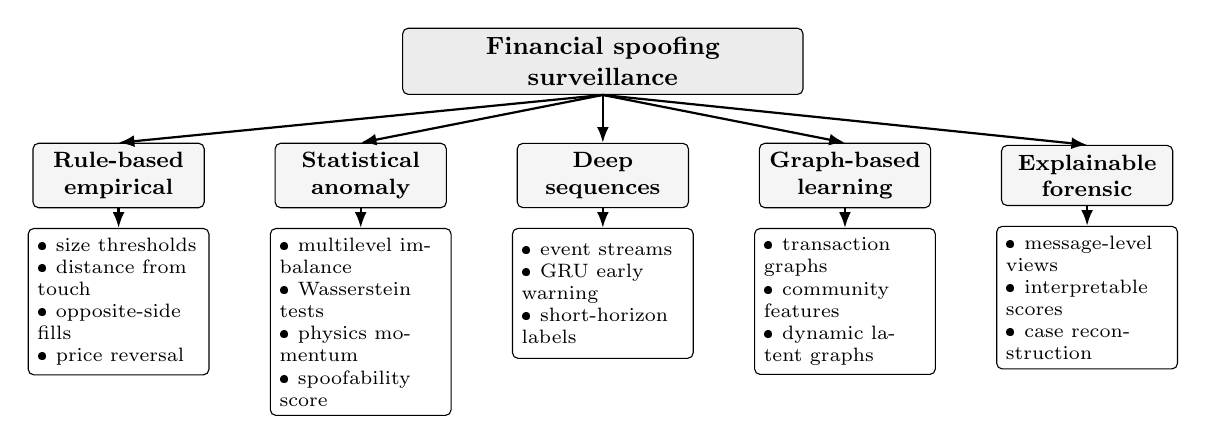
\begin{tikzpicture}[
        font=\scriptsize,
        root/.style={
            draw,
            rounded corners=2pt,
            fill=gray!15,
            align=center,
            text width=0.40\textwidth,
            minimum height=0.8cm,
            font=\small\bfseries
        },
        category/.style={
            draw,
            rounded corners=2pt,
            fill=gray!8,
            align=center,
            text width=0.16\textwidth,
            minimum height=0.75cm,
            font=\footnotesize\bfseries
        },
        detail/.style={
            draw,
            rounded corners=2pt,
            fill=white,
            align=left,
            text width=0.17\textwidth,
            minimum height=1.65cm
        },
        arrow/.style={-{Latex[length=2mm]}, thick}
    ]
        \node[root] (root) at (0,0) {Financial \mbox{spoofing} surveillance};

        \node[category] (rules) at (-6.15,-1.45) {Rule-based\\empirical};
        \node[category] (stat) at (-3.075,-1.45) {Statistical\\anomaly};
        \node[category] (seq) at (0,-1.45) {Deep\\sequences};
        \node[category] (graph) at (3.075,-1.45) {Graph-based\\learning};
        \node[category] (expl) at (6.15,-1.45) {Explainable\\forensic};

        \node[detail, below=0.25cm of rules] (rulesd) {\textbullet\ size thresholds\\\textbullet\ distance from touch\\\textbullet\ opposite-side fills\\\textbullet\ price reversal};
        \node[detail, below=0.25cm of stat] (statd) {\textbullet\ multilevel imbalance\\\textbullet\ Wasserstein tests\\\textbullet\ physics momentum\\\textbullet\ spoofability score};
        \node[detail, below=0.25cm of seq] (seqd) {\textbullet\ event streams\\\textbullet\ GRU early warning\\\textbullet\ short-horizon labels};
        \node[detail, below=0.25cm of graph] (graphd) {\textbullet\ transaction graphs\\\textbullet\ community features\\\textbullet\ dynamic latent graphs};
        \node[detail, below=0.25cm of expl] (expld) {\textbullet\ message-level views\\\textbullet\ interpretable scores\\\textbullet\ case reconstruction};

        \foreach \target in {rules,stat,seq,graph,expl} {
            \draw[arrow] (root.south) -- (\target.north);
        }
        \foreach \source/\target in {rules/rulesd,stat/statd,seq/seqd,graph/graphd,expl/expld} {
            \draw[arrow] (\source.south) -- (\target.north);
        }
    \end{tikzpicture}
    \caption{Method families in the spoofing-detection literature. The categories can overlap; each column identifies
    the main object or representation used by a strand of work.}
    \label{fig:method_taxonomy}
\end{figure}

Early empirical studies operationalize spoofing-surveillance screens through interpretable order-book conditions. Using account-level Korea Exchange
data, \cite{LeeEomPark2013} identify large orders placed far from the best quote, followed by opposite-side trading and
subsequent withdrawal. Related surveillance rules have been applied to Brazilian equities
\cite{MendoncaDeGenaro2020}, FX spot markets \cite{StenforsSusai2021}, cross-market FX activity
\cite{StenforsEtAl2023}, and Taiwan derivatives \cite{ChenHsiehYang2026}. These studies connect a screen to observable
features such as order size, posting distance, cancellation timing, opposite-side execution, and short-lived price
impact. However, the reported implementations use venue-specific thresholds, and their reconstruction can require
privileged message data or account identifiers.

A second line of work monitors statistical anomalies in the order book. \cite{TaoDayLingDrapeau2022} derive spoofing
incentives from multilevel imbalance and propose a Wasserstein-distance statistic for real-time monitoring.
\cite{LiPolukarovaVentre2023} represent the order book as a statistical-physics system and detect abnormal momentum in
cryptocurrency markets. Explainable forensic methods partly overlap with this family. Message-level visualization can
reconstruct prosecuted episodes \cite{DebieEtAl2023}. Interpretable probabilistic neural networks instead estimate how an
isolated limit order changes the conditional distribution of future prices and the expected gain from a hypothetical
manipulation strategy in centralized cryptocurrency markets \cite{FabreChallet2025}. The latter object measures
order-level \emph{spoofability}; it does not establish whether one participant generated the candidate posture, the
smaller execution-side order, and the withdrawal. Our framework addresses this complementary attribution problem by
linking these observed actions through anonymized client identifiers.

Machine-learning methods add temporal or relational structure. \cite{TuccellaNadlerSerban2021} formulate spoofing as an
early-warning problem and train a gated recurrent unit model on cryptocurrency order-book event streams. Graph-based
graph-based methods move the unit of analysis from isolated orders to networks of traders and transactions. This representation can
capture coordinated spoofing patterns \cite{KangMuNing2023,KangMuNing2024,XiangEtAl2025}. Reported models combine
temporal transaction graphs, community features, and dynamic latent representations. Their practical performance remains
difficult to compare because open labels and chronological cross-market validation are limited.

These studies imply two requirements for the present surveillance setting. First, the features must retain their
microstructure interpretation. The screen must record candidate volume, posting distance from the touch, cancellation
timing, and the relation to an opposite-side execution. Second, evaluation must reflect scarce and noisy enforcement
labels, rare positive cases, and the analyst cost of false positives. The model below therefore preserves the auditability
of rule-based surveillance while using participant-level order sequences from proprietary event data.

\section{Data}
\label{sec:data}

We use three CONSOB limit-order-book message samples. The Risanamento sample covers June--November 2024, the Nexi sample
covers 23 April 2024, and the Ferrari sample covers 13 June 2024. These samples differ in duration and participant
composition, so cross-instrument differences are descriptive rather than controlled comparisons.

For each instrument, we reconstruct the visible order book from order-level events and infer the tick size from the
reconstructed best quotes. We compute episode-conditioned metrics over the first ten book ranks. The main specification
uses a $10$-second structural post-execution window, a $2$-second rapid-withdrawal attribution window, a $2$-second
reversion horizon measured from each assigned cancellation, and a maximum candidate-order age of $90$ seconds.

One passive order can generate several child fills. We consolidate child fills into one execution cluster when they share
the passive order, client, side, price, and trading partition; consecutive fills must also be no more than $100$
milliseconds apart, with no intervening lifecycle boundary. The $100$-millisecond threshold is an operational choice, and
the reported findings are conditional on it; sensitivity to alternative inter-fill gaps is not reported here. Raw-message
identifiers and cluster memberships remain available as provenance, while execution clusters form the analytical unit for
event metrics and client--partition aggregation. The resulting surveillance dossiers support analyst review and are not
enforcement labels.

\section{Model}
\label{sec:model}
This section translates the stylized contrast between market making and spoofing into observable sequence diagnostics. We
first represent each participant's liquidity across the top $n$ book levels. We then measure whether a recent
opposite-side profile disappears after the participant's own execution and whether the associated price path is
economically consistent with the hypothesized strategy.

% \subsection{Spoofer's timeline}
% \label{subsec:spoofing_timeline}
% \begin{enumerate}
%     \item The spoofer posts a large non bona fide order far away from the best quote and, simultaneously, a small bona 
%     fide order close to the best quote
%     \item The spoofer's small order gets executed due to the price move induced by the artificially increased volume
%     on the opposite side of the book
%     \item The spoofer cancels the large non bona fide order immediately after the execution
%     \begin{figure}[htbp]
%     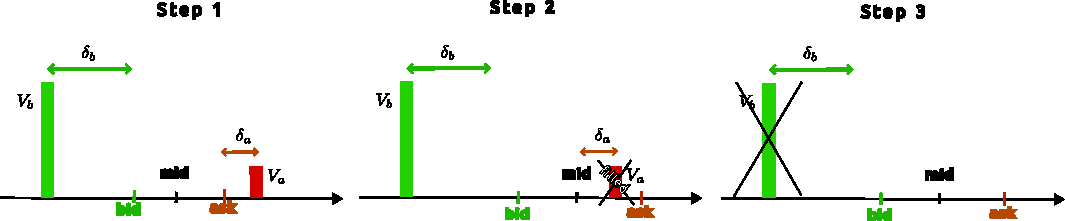
\includegraphics[width=\textwidth]{images/spoofer.pdf}
%     \caption{Timeline of a spoofing episode}
%     \end{figure}

% \end{enumerate}
% Let $i$ indicate the agent of interest, $V_a$ and $V_b$ represent the volumes of the agent's ask and bid orders, 
% respectively, and $\delta_a$ and $\delta_b$ represent their posting distances from the best quote. We consider 
% the following metric that we call distance-weighted imbalance:
% \begin{equation}
%     \left. \text{imb}_{t}^i = \frac{V_a \delta_a - V_b \delta_b}{V_a + V_b} \right|_i
% \end{equation}
% If we consider a sell intent for the spoofer, we expect $\text{imb}_{t}^i$ to be negative at step 1, to become more 
% negative at step 2, and to return to zero at step 3. The opposite holds for a buy intent.
% The crucial point is to distinguish this situation of imbalance between bid and ask from a rebalncing strategy of the market
% maker. In fact, a market maker can also post a large order on one side of the book and a small order on the other side, 
% but in this case we expect the large order to be close to the best quote and the small order to be far from the best 
% quote, while for a spoofer we seek for the opposite. Hence, in this case the imbalance would be positive and it would move
% towards zero more smoothly as the big order is filled, without a sharp and sudden jump as in the spoofer case.

\subsection{A Spatio-Temporal Framework for Spoofing Detection}
\label{sec:spoofer_timeline}

\Cref{fig:topn_spoofing_timeline} sketches the hypothesized sequence. The detector later translates each state into
observable order, execution, and cancellation records rather than inferring the participant's purpose.

\begin{figure}[htbp]
    \centering
    \resizebox{0.95\textwidth}{!}{%
    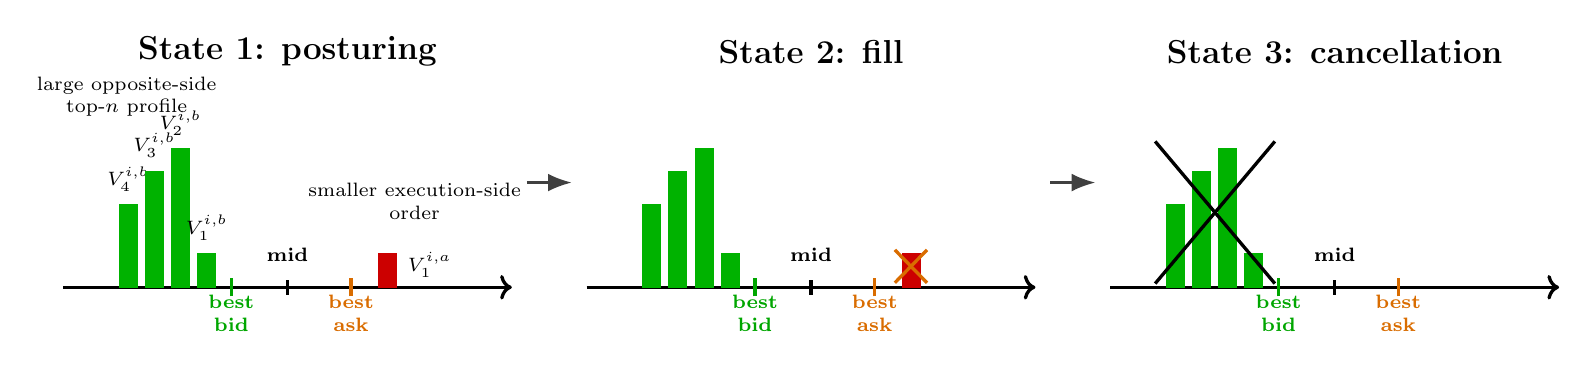
\begin{tikzpicture}[
        x=0.95cm,
        y=0.95cm,
        font=\small,
        book/.style={->, very thick},
        quote/.style={very thick},
        bid/.style={green!65!black},
        ask/.style={orange!85!black},
        fake/.style={fill=green!70!black, draw=green!70!black},
        real/.style={fill=red!80!black, draw=red!80!black},
        layer/.style={draw=black!45, fill=gray!8, rounded corners=2pt, minimum width=0.40cm},
        dist/.style={<->, black!70, very thick}
    ]
        \foreach \xshift/\step in {0/State 1: posturing,7.0/State 2: fill,14.0/State 3: cancellation} {
            \node[font=\large\bfseries] at (\xshift+3.0,3.15) {\step};
            \draw[book] (\xshift,0) -- (\xshift+6.0,0);
            \draw[quote,bid] (\xshift+2.25,-0.12) -- (\xshift+2.25,0.12)
                node[below=0.08cm, align=center, font=\scriptsize\bfseries] {best\\bid};
            \draw[quote] (\xshift+3.00,-0.10) -- (\xshift+3.00,0.10)
                node[above=0.10cm, font=\scriptsize\bfseries] {mid};
            \draw[quote,ask] (\xshift+3.85,-0.12) -- (\xshift+3.85,0.12)
                node[below=0.08cm, align=center, font=\scriptsize\bfseries] {best\\ask};
        }

        % State 1: layered bid-side deceptive profile and small ask-side bona fide order.
        \foreach \x/\h/\lab in {0.75/1.10/{$V^{i,b}_{4}$},1.10/1.55/{$V^{i,b}_{3}$},1.45/1.85/{$V^{i,b}_{2}$},1.80/0.45/{$V^{i,b}_{1}$}} {
            \draw[fake] (\x,0) rectangle +(0.24,\h);
            \node[above, font=\scriptsize] at (\x+0.12,\h+0.05) {\lab};
        }
        \draw[real] (4.22,0) rectangle +(0.24,0.45);
        \node[right, font=\scriptsize] at (4.48,0.30) {$V^{i,a}_{1}$};
        \node[align=center, font=\scriptsize] at (0.85,2.55) {large opposite-side\\top-$n$ profile};
        \node[align=center, font=\scriptsize] at (4.70,1.15) {smaller execution-side\\order};

        % State 2.
        \foreach \x/\h in {7.75/1.10,8.10/1.55,8.45/1.85,8.80/0.45} {
            \draw[fake] (\x,0) rectangle +(0.24,\h);
        }
        \draw[real] (11.22,0) rectangle +(0.24,0.45);
        \draw[orange!85!black, very thick] (11.12,0.06) -- (11.55,0.50);
        \draw[orange!85!black, very thick] (11.55,0.06) -- (11.12,0.50);


        % State 3.
        \foreach \x/\h in {14.75/1.10,15.10/1.55,15.45/1.85,15.80/0.45} {
            \draw[fake] (\x,0) rectangle +(0.24,\h);
        }
        \draw[black, very thick] (14.60,0.05) -- (16.20,1.95);
        \draw[black, very thick] (16.20,0.05) -- (14.60,1.95);


        \draw[-{Latex[length=3mm]}, thick, black!75] (6.2,1.4) -- (6.8,1.4);
        \draw[-{Latex[length=3mm]}, thick, black!75] (13.2,1.4) -- (13.8,1.4);
    \end{tikzpicture}%
    }
    \caption{Schematic top-$n$ timeline for the hypothesized spoofing mechanism. The large candidate posture forms an
    agent-specific depth profile over several bid levels, while the smaller order rests near the opposite best quote. The
    construction applies symmetrically to candidate buy- and sell-intent episodes.}
    \label{fig:topn_spoofing_timeline}
\end{figure}

The method represents a candidate episode as a conditional change in the participant's LOB footprint. A single order at
the best bid or ask does not capture this change. We instead use the participant's liquidity profile over the first $n$
price levels. This representation includes postures placed at Level 2, Level 3, or across adjacent levels, where displayed
liquidity can remain visible while facing less immediate execution risk.

The hypothesized mechanism for participant $i$ has three states:
\begin{enumerate}
    \item \textbf{State 1 (Candidate Posturing):} Shortly before the execution, the participant displays a large
    liquidity profile on one side of the book, typically away from the touch. The participant also maintains a smaller
    order near the opposite best quote.
    \item \textbf{State 2 (Execution):} The large profile is present when the smaller opposite-side order executes. In the
    hypothesized mechanism, the profile contributes mechanically to short-horizon imbalance statistics before this
    execution.
    \item \textbf{State 3 (Withdrawal):} The participant rapidly cancels the opposite-side profile after the execution,
    ending its exposure to unintended fills of those orders.
\end{enumerate}

The detector observes the sequence, not the participant's intent or the profile's causal effect on other traders. It
therefore requires the asymmetric profile to be recent, present before the fill, and withdrawn conditionally after the
fill. The recency restriction prevents long-lived liquidity on the opposite side of a later execution from entering the
candidate episode solely because it was already resting in the book.

\subsubsection{\texorpdfstring{Top-$n$}{Top-n} Participant-Specific Depth Profiles}
\label{subsec:topn_depth_profiles}

We first define the participant-specific depth profile used throughout the model. Let $s \in \{b,a\}$ denote the bid or
ask side, and let $k=1,\ldots,n$ denote book rank. Rank $k=1$ is the best quote on side $s$. For participant $i$, define
\begin{equation}
    V^{i,s}_{k}(t)
\end{equation}
as the participant's displayed volume at time $t$ on side $s$ and rank $k$. The vector
\begin{equation}
    \mathbf{V}^{i,s}_{n}(t)
    = \left(V^{i,s}_{1}(t),\ldots,V^{i,s}_{n}(t)\right)
\end{equation}
collects these quantities over the first $n$ ranks.

Raw displayed volume may not be comparable across assets or intraday periods with different market depth. The reported
implementation therefore divides participant volume by total displayed market depth at the same side and rank:
\begin{equation}
    \widetilde V^{i,s}_{k}(t)
    =
    \frac{V^{i,s}_{k}(t)}{D^{s}_{k}(t)},
    \label{eq:relative_agent_depth}
\end{equation}
where $D^{s}_{k}(t)$ is the total displayed market depth on side $s$ and rank $k$. A rank with zero market depth contributes
zero; an imbalance is undefined when the participant has no positive weighted footprint on either side.
We denote the distance from the touch by $d^{s}_{k}(t)$. In tick units, this distance equals the number of ticks between
rank $k$ and the same-side best quote, shifted upward by one. The shift gives Rank 1 a positive distance and preserves the
ordering of deeper ranks.

\subsubsection{Multilevel Distance-Weighted Imbalance}
\label{subsec:multilevel_dwi}

\paragraph{Economic intuition and a stylized parametric benchmark.}
We use a depth kernel to reduce the top-$n$ vector to a scalar weighted-liquidity measure. A high-weight rank should remain
visible to traders who process multilevel data but face relatively low immediate execution risk. The following parametric
kernel illustrates this trade-off:
\begin{equation}
    \omega^{s,\mathrm{par}}_{k}(t)
    =
    \frac{
        e^{-\lambda d^{s}_{k}(t)}
        \left(1-e^{-\kappa d^{s}_{k}(t)}\right)
    }{
        \sum_{\ell=1}^{n}
        e^{-\lambda d^{s}_{\ell}(t)}\left(
        1-e^{-\kappa d^{s}_{\ell}(t)}\right)
    },
    \label{eq:depth_kernel}
\end{equation}
The visibility component $e^{-\lambda d}$ decreases with depth. The protection component
$1-e^{-\kappa d}$ increases as the displayed price moves away from immediate execution. Their product penalizes both the
high execution risk near the touch and the lower visibility deeper in the book. The parameters $\lambda$ and $\kappa$
control the two shapes. This expression is only a conceptual benchmark: the empirical analysis uses neither these weights
nor fitted values of $\lambda$ and $\kappa$. Instead, it constructs rank-level empirical proxies for each instrument and
book side.

\Cref{fig:depth_kernel_behavior} illustrates the benchmark trade-off and its discrete normalization; it is not an
estimated empirical profile.

\begin{figure}[htbp]
    \centering
    \resizebox{0.95\textwidth}{!}{%
    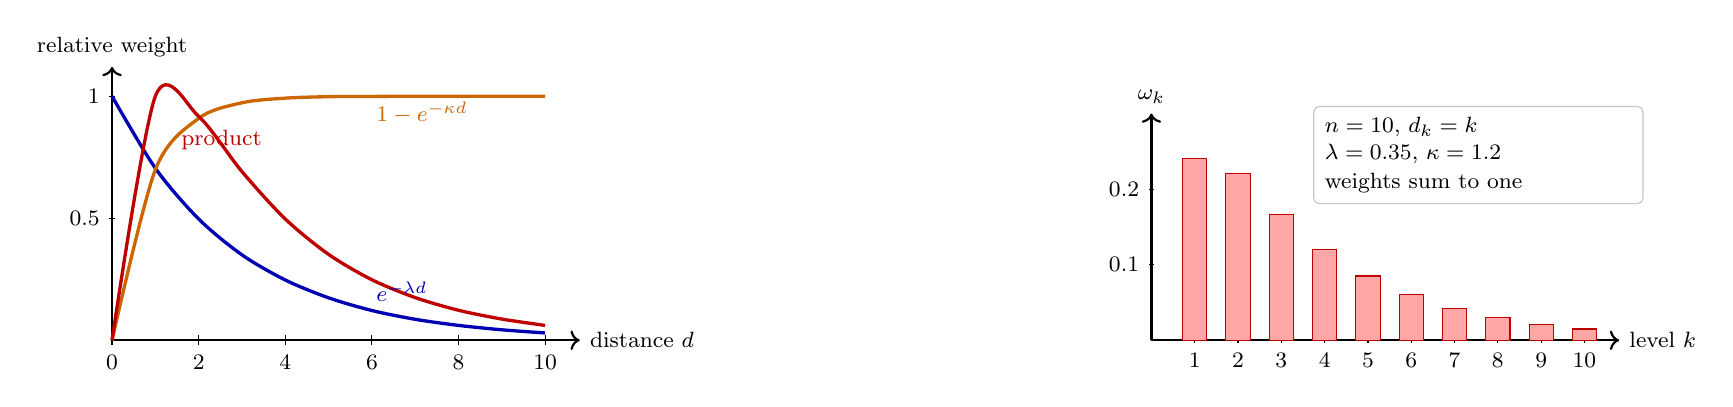
\begin{tikzpicture}[
        x=0.55cm,
        y=3.1cm,
        font=\footnotesize,
        axis/.style={->, thick},
        visibility/.style={very thick, blue!70!black},
        protection/.style={very thick, orange!80!black},
        kernel/.style={very thick, red!75!black},
        weightbar/.style={fill=red!35, draw=red!75!black},
        note/.style={draw=gray!45, rounded corners=2pt, fill=white, align=left, text width=3.9cm, inner sep=4pt}
    ]
        % Left panel: unnormalised ingredients, with the product rescaled to unit peak.
        \draw[axis] (0,0) -- (10.8,0) node[right] {distance $d$};
        \draw[axis] (0,0) -- (0,1.12) node[above, align=center] {relative weight};
        \foreach \x in {0,2,4,6,8,10} {
            \draw (\x,0.02) -- (\x,-0.02) node[below] {\x};
        }
        \foreach \y/\lab in {0.5/$0.5$,1/$1$} {
            \draw (0.06,\y) -- (-0.06,\y) node[left] {\lab};
        }

        \draw[visibility]
            plot[smooth] coordinates {(0,1.000) (1,0.705) (2,0.497) (3,0.350) (4,0.247) (5,0.174) (6,0.122) (7,0.086) (8,0.061) (9,0.043) (10,0.030)};
        \draw[protection]
            plot[smooth] coordinates {(0,0.000) (1,0.699) (2,0.909) (3,0.973) (4,0.992) (5,0.998) (6,0.999) (7,1.000) (8,1.000) (9,1.000) (10,1.000)};
        \draw[kernel]
            plot[smooth] coordinates {(0,0.000) (1,1.000) (2,0.917) (3,0.691) (4,0.497) (5,0.352) (6,0.248) (7,0.175) (8,0.123) (9,0.087) (10,0.061)};
        \node[visibility, anchor=west] at (5.85,0.20) {$e^{-\lambda d}$};
        \node[protection, anchor=west] at (5.85,0.93) {$1-e^{-\kappa d}$};
        \node[kernel, anchor=west] at (1.35,0.82) {product};

        % Right panel: discrete normalised top-n kernel weights.
        \begin{scope}[xshift=13.2cm, y=9.6cm]
            \draw[axis] (0,0) -- (10.8,0) node[right] {level $k$};
            \draw[axis] (0,0) -- (0,0.30) node[above] {$\omega_k$};
            \foreach \x in {1,2,3,4,5,6,7,8,9,10} {
                \draw (\x,0.004) -- (\x,-0.004) node[below] {\x};
            }
            \foreach \y/\lab in {0.1/$0.1$,0.2/$0.2$} {
                \draw (0.06,\y) -- (-0.06,\y) node[left] {\lab};
            }
            \foreach \x/\h in {1/0.241,2/0.221,3/0.166,4/0.120,5/0.085,6/0.060,7/0.042,8/0.030,9/0.021,10/0.015} {
                \draw[weightbar] (\x-0.28,0) rectangle (\x+0.28,\h);
            }
            \node[note] at (7.55,0.245)
            {$n=10$, $d_k=k$\\
            $\lambda=0.35$, $\kappa=1.2$\\[1pt]
            weights sum to one};
        \end{scope}
    \end{tikzpicture}%
    }
    \caption{Conceptual depth kernel in \cref{eq:depth_kernel}. The left panel shows decreasing visibility, increasing
    protection from immediate execution, and their product. The right panel shows normalized weights for one illustrative
    parameter choice. The empirical analysis uses the instrument- and side-specific kernel in
    \cref{eq:empirical_depth_kernel}, not these parametric weights.}
    \label{fig:depth_kernel_behavior}
\end{figure}

\paragraph{Operational empirical depth kernel.}
The operational kernel replaces both exponential components with empirical rank-level quantities. We calibrate each book
rank $k$ separately for instrument $m$ and side $s$. A rank receives more weight when its depth has a strong short-horizon
association with mid-price changes and its displayed price is rarely reached over the same horizon. Tick distance can vary
for a given rank over time, but the calibrated unit remains the rank.

\emph{Operational calculation.} We reconstruct a post-event top-$n$ snapshot after every ordered message. Let
$\mathcal{O}_{m,s,k}$ contain the snapshots in which rank $k$ exists on side $s$ and has positive displayed depth. For
each $t\in\mathcal{O}_{m,s,k}$, the indicator $R^{m,s}_{t,k}(H)$ equals one when at least one fill during $(t,t+H]$ occurs
at or through the rank's displayed price. An ask rank is reached when the maximum ask fill price in the window is at least
the displayed price. A bid rank is reached when the minimum bid fill price is at most the displayed price. We estimate the
rank-level hit probability from pooled hit and exposure counts:
\begin{equation}
    \widehat p^{m,s}_{k}(H)
    =
    \frac{
        \sum_{t\in\mathcal{O}_{m,s,k}}R^{m,s}_{t,k}(H)
    }{
        |\mathcal{O}_{m,s,k}|
    }.
    \label{eq:empirical_hit_probability}
\end{equation}
Each observable snapshot contributes once, even when the same rank appears at different tick distances. Thus,
\cref{eq:empirical_hit_probability} divides total hits by total exposures; it does not average distance-specific hit
rates. Realized tick distance is retained only as descriptive metadata and does not define additional kernel rows or enter
a parametric fit. The estimator is a short-horizon proxy for whether the displayed price is reached. It is not an
individual order's fill probability, which also depends on queue position, order size, and intervening cancellations.
We define the protection component as the complement of the hit probability:
\begin{equation}
    \widehat\rho^{m,s}_{k}(H)=1-\widehat p^{m,s}_{k}(H),
    \label{eq:empirical_protection_profile}
\end{equation}
A value of $\widehat\rho^{m,s}_{k}(H)$ near one indicates that rank $k$ is rarely reached over horizon $H$.

The second component measures the association between displayed depth and subsequent short-horizon price changes. Let
$D^{m,s}_{k}(t)$ denote total market depth, rather than participant-$i$ depth, at rank $k$. Total displayed top-$n$ depth
at snapshot $t$ is
\begin{equation}
    D^{m}_{n}(t)
    =
    \sum_{r=1}^{n}\left(D^{m,a}_{r}(t)+D^{m,b}_{r}(t)\right).
    \label{eq:total_topn_market_depth}
\end{equation}
We then define the signed and normalized contribution of side $s$ and rank $k$:
\begin{equation}
    Z^{m,s}_{t,k}
    =
    \sigma_s\frac{D^{m,s}_{k}(t)}{D^{m}_{n}(t)},
    \qquad
    \sigma_s= \begin{cases}
        +1, & s=ask,\\
        -1, & s=bid.
    \end{cases}
    \label{eq:normalized_level_contribution}
\end{equation}
The magnitude $|Z^{m,s}_{t,k}|$ is the fraction of visible top-$n$ depth supplied by that side and rank. The sign makes ask
and bid depth contribute in opposite directions to imbalance.

For each snapshot, $M^m_{t,H}$ is the last finite reconstructed mid-price observed after $t$ and no later than $t+H$.
The corresponding price change is $\Delta M^m_{t,H}=M^m_{t,H}-M^m(t)$. Let $\mathcal{V}_{m,s,k}(H)$ contain the rank-$k$
snapshots for which both mid-prices are finite. For each instrument--side--rank cell, we compute the following pooled
population covariance in absolute value, where the overbars denote sample means over
$\mathcal{V}_{m,s,k}(H)$:
\begin{equation}
    \widehat\nu^{m,s}_{k}(H)
    =
    \left|
        \frac{1}{|\mathcal{V}_{m,s,k}(H)|}
        \sum_{t\in\mathcal{V}_{m,s,k}(H)}
        \left(Z^{m,s}_{t,k}-\overline Z^{m,s}_{k}\right)
        \left(\Delta M^m_{t,H}-\overline{\Delta M}^{m,s}_{k,H}\right)
    \right|.
    \label{eq:empirical_visibility_covariance}
\end{equation}
The absolute value makes $\widehat\nu^{m,s}_{k}(H)$ a measure of the magnitude, rather than the direction, of
rank-specific co-movement. We pool observations across realized tick distances before computing the covariance. We do not
compute or average separate distance-bucket covariances. This quantity is a weighting proxy, not a causal estimate of price
impact. It is also expressed in instrument-specific price units. We therefore use it only to allocate weights across
ranks on the same side of one instrument, not to compare covariance magnitudes across instruments.

The empirical kernel follows the same multiplicative decomposition as \cref{eq:depth_kernel}, but no exponential curve is
fitted. Before normalization, we apply a zero floor to protection and a $10^{-12}$ floor to the absolute covariance:
\begin{equation}
    \widetilde\rho^{m,s}_{k}(H)=\max\{1-\widehat p^{m,s}_{k}(H),0\},
    \qquad
    \widetilde\nu^{m,s}_{k}(H)=\max\{\widehat\nu^{m,s}_{k}(H),10^{-12}\},
    \label{eq:empirical_kernel_floors}
\end{equation}
We normalize the product of these two quantities within each instrument and side:
\begin{equation}
    \widehat\omega^{m,s}_{k}(H)
    =
    \frac{
        \widetilde\nu^{m,s}_{k}(H)\,\widetilde\rho^{m,s}_{k}(H)
    }{
        \sum_{\ell=1}^{n}\widetilde\nu^{m,s}_{\ell}(H)\,\widetilde\rho^{m,s}_{\ell}(H)
    }.
    \label{eq:empirical_depth_kernel}
\end{equation}
The denominator must be finite and strictly positive. If every rank on a side has zero protection, or if the product is
otherwise degenerate, calibration fails instead of returning an uninterpretable all-zero vector. Every reported kernel in
\cref{tab:empirical_depth_kernel_calibration} passes this condition and sums to one before rounding. A rank therefore
receives high weight only when it combines price association with low short-horizon execution risk.

In the remaining formulas, the operational value of $\omega^{s}_{k}(t)$ is
$\widehat\omega^{m,s}_{k}(H)$. Every event for instrument $m$ uses the same calibrated kernel. The kernel is not
re-estimated by client, event, or observed outcome. Calibration produces one row for each $(m,s,k)$ cell, and the runtime
loader rejects duplicate rank rows instead of resolving them by row order. The descriptive analysis uses the full
available sample for each instrument. A prospective or out-of-sample application must instead estimate the kernel on an
earlier training period and hold it fixed, so that future order flow does not enter the weights.

\begin{table}[htbp]
\centering
\caption{Operational full-sample empirical top-$10$ depth-kernel weights at horizon $H=10$ seconds. Values are rounded to
three decimal places and sum to one within each instrument and side before rounding. These weights, rather than fitted
exponential parameters, enter the empirical spoofing metrics.}
\label{tab:empirical_depth_kernel_calibration}
\scriptsize
\setlength{\tabcolsep}{1.7pt}
\begin{tabular}{ll*{10}{r}}
\toprule
Instrument & Side & $\widehat\omega_1$ & $\widehat\omega_2$ & $\widehat\omega_3$ & $\widehat\omega_4$ & $\widehat\omega_5$ & $\widehat\omega_6$ & $\widehat\omega_7$ & $\widehat\omega_8$ & $\widehat\omega_9$ & $\widehat\omega_{10}$ \\
\midrule
Risanamento & Ask & 0.127 & 0.248 & 0.348 & 0.062 & 0.004 & 0.039 & 0.018 & 0.012 & 0.078 & 0.064 \\
             & Bid & 0.526 & 0.012 & 0.019 & 0.146 & 0.091 & 0.065 & 0.082 & 0.034 & 0.002 & 0.024 \\
Nexi        & Ask & 0.028 & 0.069 & 0.033 & 0.138 & 0.225 & 0.149 & 0.275 & 0.011 & 0.020 & 0.051 \\
             & Bid & 0.045 & 0.166 & 0.184 & 0.276 & 0.165 & 0.033 & 0.006 & 0.052 & 0.064 & 0.008 \\
Ferrari     & Ask & 0.095 & 0.022 & 0.016 & 0.209 & 0.270 & 0.032 & 0.144 & 0.032 & 0.033 & 0.147 \\
             & Bid & 0.148 & 0.107 & 0.007 & 0.054 & 0.072 & 0.197 & 0.102 & 0.038 & 0.176 & 0.100 \\
\bottomrule
\end{tabular}
\end{table}

The operational calibration uses the first ten ranks and the same $H=10$ second horizon for every instrument. It produces
20 weights per instrument, one for each side--rank cell. The kernel remains side-specific. To draw one curve per
instrument for visualization only, we average the bid and ask weights at each rank:
\begin{equation}
    \overline{\omega}^{m}_{k}(H)
    =
    \frac{1}{2}\left(
        \widehat\omega^{m,a}_{k}(H)
        +
        \widehat\omega^{m,b}_{k}(H)
    \right).
    \label{eq:side_averaged_empirical_kernel}
\end{equation}
Each side-specific kernel sums to one, so $\sum_{k=1}^{10}\overline{\omega}^{m}_{k}(H)=1$. We use this average only in
\cref{fig:empirical_top10_kernel_profiles}. The empirical surveillance metrics use the side-specific top-$10$ weights in
\cref{tab:empirical_depth_kernel_calibration}.

\begin{figure}[htbp]
    \centering
    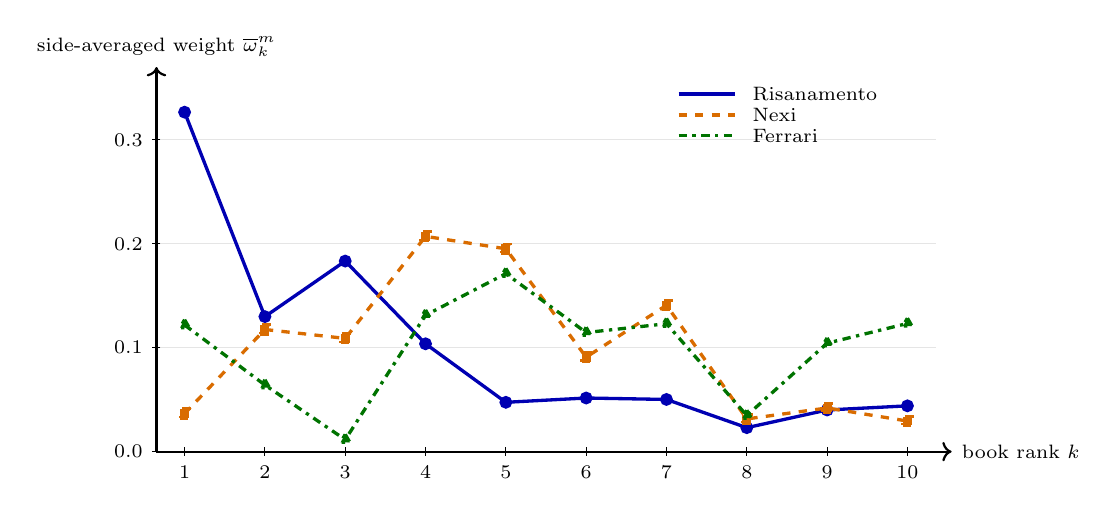
\begin{tikzpicture}[
        x=1.02cm,
        y=13.2cm,
        font=\scriptsize,
        axis/.style={->, thick},
        grid/.style={gray!20, thin},
        risanamento/.style={blue!70!black, very thick, mark=*, mark size=1.7pt},
        nexi/.style={orange!85!black, very thick, dashed, mark=square*, mark size=1.6pt},
        ferrari/.style={green!45!black, very thick, dash dot, mark=triangle*, mark size=1.9pt}
    ]
        \foreach \y in {0.1,0.2,0.3} {
            \draw[grid] (0.65,\y) -- (10.35,\y);
        }
        \draw[axis] (0.65,0) -- (10.55,0) node[right] {book rank $k$};
        \draw[axis] (0.65,0) -- (0.65,0.37) node[above, align=center]
            {side-averaged weight $\overline{\omega}^{m}_{k}$};

        \foreach \x in {1,...,10} {
            \draw (\x,0.004) -- (\x,-0.004) node[below] {\x};
        }
        \foreach \y/\lab in {0.0/$0.0$,0.1/$0.1$,0.2/$0.2$,0.3/$0.3$} {
            \draw (0.70,\y) -- (0.60,\y) node[left] {\lab};
        }

        \draw[risanamento]
            plot coordinates {
                (1,0.326590) (2,0.129904) (3,0.183346) (4,0.103747) (5,0.047449)
                (6,0.051590) (7,0.050207) (8,0.023040) (9,0.040075) (10,0.044052)
            };
        \draw[nexi]
            plot coordinates {
                (1,0.036660) (2,0.117508) (3,0.108946) (4,0.207104) (5,0.195161)
                (6,0.090903) (7,0.140818) (8,0.031470) (9,0.042001) (10,0.029429)
            };
        \draw[ferrari]
            plot coordinates {
                (1,0.121867) (2,0.064095) (3,0.011556) (4,0.131256) (5,0.171245)
                (6,0.114549) (7,0.123072) (8,0.034722) (9,0.104320) (10,0.123319)
            };

        \draw[risanamento] (7.15,0.344) -- (7.85,0.344);
        \node[anchor=west] at (7.95,0.344) {Risanamento};
        \draw[nexi] (7.15,0.324) -- (7.85,0.324);
        \node[anchor=west] at (7.95,0.324) {Nexi};
        \draw[ferrari] (7.15,0.304) -- (7.85,0.304);
        \node[anchor=west] at (7.95,0.304) {Ferrari};
    \end{tikzpicture}
    \caption{Full-sample empirical top-$10$ depth-kernel profiles at $H=10$ seconds. Each line is the arithmetic mean of
    the separately normalized bid and ask weights in \cref{eq:side_averaged_empirical_kernel}. The mean permits one curve
    per instrument on a common rank axis and is used only for visualization. Surveillance metrics use the underlying
    side-specific kernels.}
    \label{fig:empirical_top10_kernel_profiles}
\end{figure}

To expose the two empirical inputs rather than only their normalized product,
\Cref{fig:empirical_topn_visibility_profiles,fig:empirical_topn_execution_risk_profiles} plot the side-specific
visibility and execution-risk profiles used in the calibration. The second plot reports $p_k^{i,s}$ directly; the
kernel uses its protection complement $\rho_k^{i,s}=1-p_k^{i,s}$.

% Generated by scripts/generate_empirical_kernel_component_figures.py; do not edit manually.
% calibration root: outputs/depth_kernel_calibration/20260717_145624_rank_pooled_top10_h10
% source RISANAMENTO: outputs/depth_kernel_calibration/20260717_145624_rank_pooled_top10_h10/RISANAMENTO_top10_h10/empirical_depth_kernel.csv sha256=6ecb2071cf524f6090dff6596dc64248cbf59af2c55cf0d33e0649fcc52abe45
% source NEXI: outputs/depth_kernel_calibration/20260717_145624_rank_pooled_top10_h10/NEXI_top10_h10/empirical_depth_kernel.csv sha256=deaeb5a1c7a301d48c51347fbc4bdc2dc389281302aeb41192c20190920335f5
% source FERRARI: outputs/depth_kernel_calibration/20260717_145624_rank_pooled_top10_h10/FERRARI_top10_h10/empirical_depth_kernel.csv sha256=d5fdc562b059874471a511f2990341ceed08f434ddefb8b3cf31589979a67540

% data column: visibility_component
\begin{figure}[!ht]
\centering
\resizebox{\textwidth}{!}{%
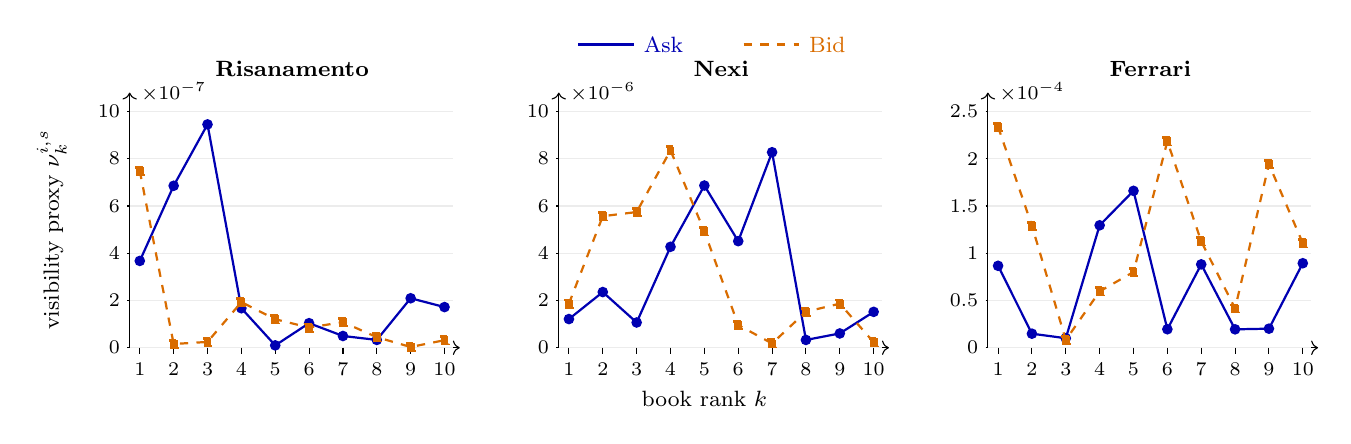
\begin{tikzpicture}
\begin{scope}[xshift=0.00cm]
\begin{scope}[x=0.43cm,y=0.30000000cm]
  \draw[->] (0.7,0) -- (10.45,0);
  \draw[->] (0.7,0) -- (0.7,10.8);
  \draw[gray!15] (0.7,0) -- (10.25,0);
  \draw (0.63,0) -- (0.7,0) node[left,font=\scriptsize] {0};
  \draw[gray!15] (0.7,2) -- (10.25,2);
  \draw (0.63,2) -- (0.7,2) node[left,font=\scriptsize] {2};
  \draw[gray!15] (0.7,4) -- (10.25,4);
  \draw (0.63,4) -- (0.7,4) node[left,font=\scriptsize] {4};
  \draw[gray!15] (0.7,6) -- (10.25,6);
  \draw (0.63,6) -- (0.7,6) node[left,font=\scriptsize] {6};
  \draw[gray!15] (0.7,8) -- (10.25,8);
  \draw (0.63,8) -- (0.7,8) node[left,font=\scriptsize] {8};
  \draw[gray!15] (0.7,10) -- (10.25,10);
  \draw (0.63,10) -- (0.7,10) node[left,font=\scriptsize] {10};
  \draw (1,0) -- (1,-0.025 * 10) node[below,font=\scriptsize] {1};
  \draw (2,0) -- (2,-0.025 * 10) node[below,font=\scriptsize] {2};
  \draw (3,0) -- (3,-0.025 * 10) node[below,font=\scriptsize] {3};
  \draw (4,0) -- (4,-0.025 * 10) node[below,font=\scriptsize] {4};
  \draw (5,0) -- (5,-0.025 * 10) node[below,font=\scriptsize] {5};
  \draw (6,0) -- (6,-0.025 * 10) node[below,font=\scriptsize] {6};
  \draw (7,0) -- (7,-0.025 * 10) node[below,font=\scriptsize] {7};
  \draw (8,0) -- (8,-0.025 * 10) node[below,font=\scriptsize] {8};
  \draw (9,0) -- (9,-0.025 * 10) node[below,font=\scriptsize] {9};
  \draw (10,0) -- (10,-0.025 * 10) node[below,font=\scriptsize] {10};
  \node[anchor=south west,font=\scriptsize] at (0.75,10) {$\times 10^{-7}$};
  \node[rotate=90,font=\footnotesize] at (-1.6,5) {visibility proxy $\nu_k^{i,s}$};
  \node[font=\footnotesize\bfseries] at (5.5,11.8) {Risanamento};
  \draw[blue!70!black, thick, mark=*, mark size=1.5pt] plot coordinates {(1,3.675229767983178) (2,6.855802152861837) (3,9.454395390358135) (4,1.6711452429542564) (5,0.09967103872544607) (6,1.03986078936913) (7,0.49722130939049286) (8,0.331027311346062) (9,2.094561089973038) (10,1.7209334991488594)};
  % RISANAMENTO ask visibility_component raw: 1:3.6752297679831775e-07, 2:6.855802152861836e-07, 3:9.4543953903581345e-07, 4:1.6711452429542563e-07, 5:9.9671038725446058e-09, 6:1.03986078936913e-07, 7:4.9722130939049281e-08, 8:3.31027311346062e-08, 9:2.0945610899730381e-07, 10:1.7209334991488592e-07
  \draw[orange!85!black, thick, dashed, mark=square*, mark size=1.4pt] plot coordinates {(1,7.4850054933810215) (2,0.15725764971410325) (3,0.24659322933232064) (4,1.930205433978854) (5,1.2069432758813796) (6,0.8540517059063696) (7,1.0836250920231838) (8,0.4466903180509029) (9,0.031098089940439774) (10,0.31967530278917544)};
  % RISANAMENTO bid visibility_component raw: 1:7.4850054933810209e-07, 2:1.5725764971410324e-08, 3:2.4659322933232062e-08, 4:1.9302054339788539e-07, 5:1.2069432758813797e-07, 6:8.5405170590636958e-08, 7:1.0836250920231838e-07, 8:4.4669031805090292e-08, 9:3.1098089940439771e-09, 10:3.1967530278917541e-08
\end{scope}
\end{scope}
\begin{scope}[xshift=5.45cm]
\begin{scope}[x=0.43cm,y=0.30000000cm]
  \draw[->] (0.7,0) -- (10.45,0);
  \draw[->] (0.7,0) -- (0.7,10.8);
  \draw[gray!15] (0.7,0) -- (10.25,0);
  \draw (0.63,0) -- (0.7,0) node[left,font=\scriptsize] {0};
  \draw[gray!15] (0.7,2) -- (10.25,2);
  \draw (0.63,2) -- (0.7,2) node[left,font=\scriptsize] {2};
  \draw[gray!15] (0.7,4) -- (10.25,4);
  \draw (0.63,4) -- (0.7,4) node[left,font=\scriptsize] {4};
  \draw[gray!15] (0.7,6) -- (10.25,6);
  \draw (0.63,6) -- (0.7,6) node[left,font=\scriptsize] {6};
  \draw[gray!15] (0.7,8) -- (10.25,8);
  \draw (0.63,8) -- (0.7,8) node[left,font=\scriptsize] {8};
  \draw[gray!15] (0.7,10) -- (10.25,10);
  \draw (0.63,10) -- (0.7,10) node[left,font=\scriptsize] {10};
  \draw (1,0) -- (1,-0.025 * 10) node[below,font=\scriptsize] {1};
  \draw (2,0) -- (2,-0.025 * 10) node[below,font=\scriptsize] {2};
  \draw (3,0) -- (3,-0.025 * 10) node[below,font=\scriptsize] {3};
  \draw (4,0) -- (4,-0.025 * 10) node[below,font=\scriptsize] {4};
  \draw (5,0) -- (5,-0.025 * 10) node[below,font=\scriptsize] {5};
  \draw (6,0) -- (6,-0.025 * 10) node[below,font=\scriptsize] {6};
  \draw (7,0) -- (7,-0.025 * 10) node[below,font=\scriptsize] {7};
  \draw (8,0) -- (8,-0.025 * 10) node[below,font=\scriptsize] {8};
  \draw (9,0) -- (9,-0.025 * 10) node[below,font=\scriptsize] {9};
  \draw (10,0) -- (10,-0.025 * 10) node[below,font=\scriptsize] {10};
  \node[anchor=south west,font=\scriptsize] at (0.75,10) {$\times 10^{-6}$};
  \node[font=\footnotesize\bfseries] at (5.5,11.8) {Nexi};
  \draw[blue!70!black, thick, mark=*, mark size=1.5pt] plot coordinates {(1,1.2138032154980023) (2,2.357195510456608) (3,1.0685006264223715) (4,4.273217243409157) (5,6.866026041374058) (6,4.512030446576142) (7,8.275878917434618) (8,0.32997233355025435) (9,0.6049414509297961) (10,1.5188249155682871)};
  % NEXI ask visibility_component raw: 1:1.2138032154980023e-06, 2:2.357195510456608e-06, 3:1.0685006264223715e-06, 4:4.2732172434091567e-06, 5:6.8660260413740573e-06, 6:4.5120304465761415e-06, 7:8.2758789174346172e-06, 8:3.2997233355025434e-07, 9:6.0494145092979615e-07, 10:1.5188249155682871e-06
  \draw[orange!85!black, thick, dashed, mark=square*, mark size=1.4pt] plot coordinates {(1,1.8674773855957816) (2,5.568884213770531) (3,5.7442838166896815) (4,8.353844420062963) (5,4.925771459538285) (6,0.9619962140487628) (7,0.1805094913160257) (8,1.5237267589959187) (9,1.8662709068477343) (10,0.2317283350241909)};
  % NEXI bid visibility_component raw: 1:1.8674773855957815e-06, 2:5.5688842137705302e-06, 3:5.7442838166896813e-06, 4:8.3538444200629627e-06, 5:4.9257714595382846e-06, 6:9.6199621404876272e-07, 7:1.8050949131602569e-07, 8:1.5237267589959187e-06, 9:1.8662709068477342e-06, 10:2.3172833502419091e-07
\end{scope}
\end{scope}
\begin{scope}[xshift=10.90cm]
\begin{scope}[x=0.43cm,y=1.20000000cm]
  \draw[->] (0.7,0) -- (10.45,0);
  \draw[->] (0.7,0) -- (0.7,2.7);
  \draw[gray!15] (0.7,0) -- (10.25,0);
  \draw (0.63,0) -- (0.7,0) node[left,font=\scriptsize] {0};
  \draw[gray!15] (0.7,0.5) -- (10.25,0.5);
  \draw (0.63,0.5) -- (0.7,0.5) node[left,font=\scriptsize] {0.5};
  \draw[gray!15] (0.7,1) -- (10.25,1);
  \draw (0.63,1) -- (0.7,1) node[left,font=\scriptsize] {1};
  \draw[gray!15] (0.7,1.5) -- (10.25,1.5);
  \draw (0.63,1.5) -- (0.7,1.5) node[left,font=\scriptsize] {1.5};
  \draw[gray!15] (0.7,2) -- (10.25,2);
  \draw (0.63,2) -- (0.7,2) node[left,font=\scriptsize] {2};
  \draw[gray!15] (0.7,2.5) -- (10.25,2.5);
  \draw (0.63,2.5) -- (0.7,2.5) node[left,font=\scriptsize] {2.5};
  \draw (1,0) -- (1,-0.025 * 2.5) node[below,font=\scriptsize] {1};
  \draw (2,0) -- (2,-0.025 * 2.5) node[below,font=\scriptsize] {2};
  \draw (3,0) -- (3,-0.025 * 2.5) node[below,font=\scriptsize] {3};
  \draw (4,0) -- (4,-0.025 * 2.5) node[below,font=\scriptsize] {4};
  \draw (5,0) -- (5,-0.025 * 2.5) node[below,font=\scriptsize] {5};
  \draw (6,0) -- (6,-0.025 * 2.5) node[below,font=\scriptsize] {6};
  \draw (7,0) -- (7,-0.025 * 2.5) node[below,font=\scriptsize] {7};
  \draw (8,0) -- (8,-0.025 * 2.5) node[below,font=\scriptsize] {8};
  \draw (9,0) -- (9,-0.025 * 2.5) node[below,font=\scriptsize] {9};
  \draw (10,0) -- (10,-0.025 * 2.5) node[below,font=\scriptsize] {10};
  \node[anchor=south west,font=\scriptsize] at (0.75,2.5) {$\times 10^{-4}$};
  \node[font=\footnotesize\bfseries] at (5.5,2.95) {Ferrari};
  \draw[blue!70!black, thick, mark=*, mark size=1.5pt] plot coordinates {(1,0.8669505020816368) (2,0.1485759198632677) (3,0.10059702674753057) (4,1.2956601892544413) (5,1.6603869526647457) (6,0.19557846353831482) (7,0.8821362998985953) (8,0.19476684019606572) (9,0.20169455861968041) (10,0.8943935007246941)};
  % FERRARI ask visibility_component raw: 1:8.6695050208163686e-05, 2:1.485759198632677e-05, 3:1.0059702674753058e-05, 4:0.00012956601892544412, 5:0.00016603869526647457, 6:1.9557846353831483e-05, 7:8.8213629989859532e-05, 8:1.9476684019606572e-05, 9:2.0169455861968043e-05, 10:8.9439350072469421e-05
  \draw[orange!85!black, thick, dashed, mark=square*, mark size=1.4pt] plot coordinates {(1,2.338679183565612) (2,1.291355118638466) (3,0.08201799287649617) (4,0.5966462138610819) (5,0.8015132512207448) (6,2.184977047983166) (7,1.1257505456756975) (8,0.41537003587522076) (9,1.9429973087449643) (10,1.1061392811485924)};
  % FERRARI bid visibility_component raw: 1:0.0002338679183565612, 2:0.00012913551186384661, 3:8.2017992876496163e-06, 4:5.9664621386108187e-05, 5:8.0151325122074484e-05, 6:0.00021849770479831661, 7:0.00011257505456756977, 8:4.1537003587522077e-05, 9:0.00019429973087449644, 10:0.00011061392811485925
\end{scope}
\end{scope}
\node[font=\footnotesize] at (7.6,-0.65) {book rank $k$};
\draw[blue!70!black,thick,mark=*,mark size=1.5pt] (6.0,3.85) -- (6.7,3.85) node[right,font=\footnotesize] {Ask};
\draw[orange!85!black,thick,dashed,mark=square*,mark size=1.4pt] (8.1,3.85) -- (8.8,3.85) node[right,font=\footnotesize] {Bid};
\end{tikzpicture}%
}
\caption{Side-specific empirical visibility proxy by book rank. Each panel shows the stored \texttt{visibility\_component} values from the full-sample top-$10$, $h=10$-second calibration. Separate axis multipliers preserve the instrument-specific price units; vertical magnitudes should not be compared across instruments.}
\label{fig:empirical_topn_visibility_profiles}
\end{figure}

% data column: hit_probability; protection_component = 1 - hit_probability
\begin{figure}[!ht]
\centering
\resizebox{\textwidth}{!}{%
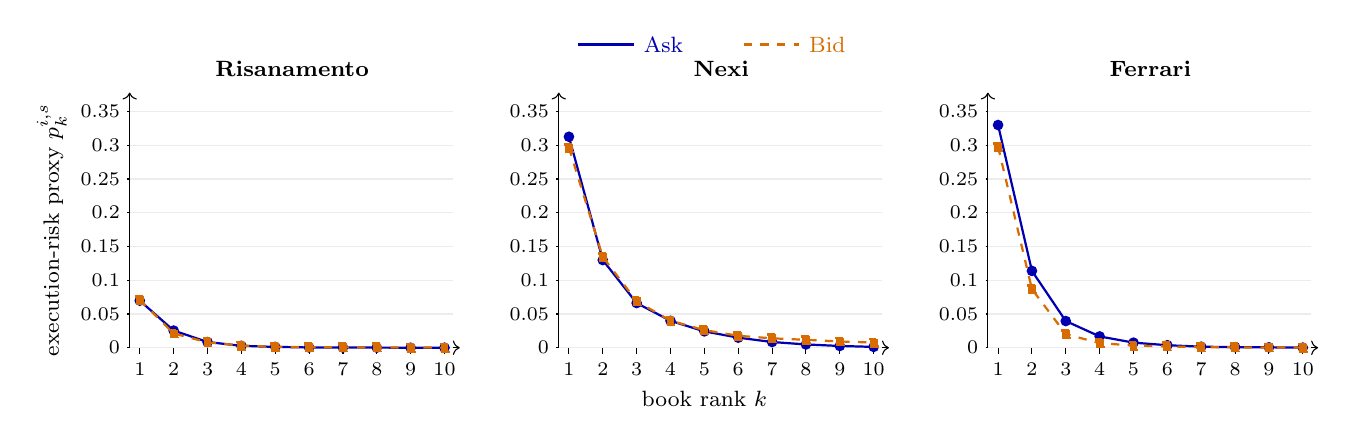
\begin{tikzpicture}
\begin{scope}[xshift=0.00cm]
\begin{scope}[x=0.43cm,y=8.57142857cm]
  \draw[->] (0.7,0) -- (10.45,0);
  \draw[->] (0.7,0) -- (0.7,0.378);
  \draw[gray!15] (0.7,0) -- (10.25,0);
  \draw (0.63,0) -- (0.7,0) node[left,font=\scriptsize] {0};
  \draw[gray!15] (0.7,0.05) -- (10.25,0.05);
  \draw (0.63,0.05) -- (0.7,0.05) node[left,font=\scriptsize] {0.05};
  \draw[gray!15] (0.7,0.1) -- (10.25,0.1);
  \draw (0.63,0.1) -- (0.7,0.1) node[left,font=\scriptsize] {0.1};
  \draw[gray!15] (0.7,0.15) -- (10.25,0.15);
  \draw (0.63,0.15) -- (0.7,0.15) node[left,font=\scriptsize] {0.15};
  \draw[gray!15] (0.7,0.2) -- (10.25,0.2);
  \draw (0.63,0.2) -- (0.7,0.2) node[left,font=\scriptsize] {0.2};
  \draw[gray!15] (0.7,0.25) -- (10.25,0.25);
  \draw (0.63,0.25) -- (0.7,0.25) node[left,font=\scriptsize] {0.25};
  \draw[gray!15] (0.7,0.3) -- (10.25,0.3);
  \draw (0.63,0.3) -- (0.7,0.3) node[left,font=\scriptsize] {0.3};
  \draw[gray!15] (0.7,0.35) -- (10.25,0.35);
  \draw (0.63,0.35) -- (0.7,0.35) node[left,font=\scriptsize] {0.35};
  \draw (1,0) -- (1,-0.025 * 0.35) node[below,font=\scriptsize] {1};
  \draw (2,0) -- (2,-0.025 * 0.35) node[below,font=\scriptsize] {2};
  \draw (3,0) -- (3,-0.025 * 0.35) node[below,font=\scriptsize] {3};
  \draw (4,0) -- (4,-0.025 * 0.35) node[below,font=\scriptsize] {4};
  \draw (5,0) -- (5,-0.025 * 0.35) node[below,font=\scriptsize] {5};
  \draw (6,0) -- (6,-0.025 * 0.35) node[below,font=\scriptsize] {6};
  \draw (7,0) -- (7,-0.025 * 0.35) node[below,font=\scriptsize] {7};
  \draw (8,0) -- (8,-0.025 * 0.35) node[below,font=\scriptsize] {8};
  \draw (9,0) -- (9,-0.025 * 0.35) node[below,font=\scriptsize] {9};
  \draw (10,0) -- (10,-0.025 * 0.35) node[below,font=\scriptsize] {10};
  \node[rotate=90,font=\footnotesize] at (-1.6,0.175) {execution-risk proxy $p_k^{i,s}$};
  \node[font=\footnotesize\bfseries] at (5.5,0.413) {Risanamento};
  \draw[blue!70!black, thick, mark=*, mark size=1.5pt] plot coordinates {(1,0.06972349940165018) (2,0.02545533573561784) (3,0.008478028770510227) (4,0.0028297304716921367) (5,0.0012412635498727) (6,0.0004097636793952453) (7,0.0002830315509421413) (8,0.00021971635327554557) (9,0.0) (10,0.0)};
  % RISANAMENTO ask hit_probability raw: 1:0.06972349940165018, 2:0.02545533573561784, 3:0.0084780287705102271, 4:0.0028297304716921367, 5:0.0012412635498726999, 6:0.0004097636793952453, 7:0.0002830315509421413, 8:0.00021971635327554557, 9:0, 10:0
  \draw[orange!85!black, thick, dashed, mark=square*, mark size=1.4pt] plot coordinates {(1,0.07096878130100093) (2,0.021101548570064722) (3,0.007994257645916313) (4,0.0031324298201674864) (5,0.0014088794806261372) (6,0.0008309423027754893) (7,0.0005630550368480321) (8,0.0003863103073313112) (9,0.00020106276030446647) (10,0.00018748873264827834)};
  % RISANAMENTO bid hit_probability raw: 1:0.070968781301000927, 2:0.021101548570064722, 3:0.0079942576459163129, 4:0.0031324298201674864, 5:0.0014088794806261372, 6:0.00083094230277548935, 7:0.00056305503684803214, 8:0.00038631030733131118, 9:0.00020106276030446647, 10:0.00018748873264827834
\end{scope}
\end{scope}
\begin{scope}[xshift=5.45cm]
\begin{scope}[x=0.43cm,y=8.57142857cm]
  \draw[->] (0.7,0) -- (10.45,0);
  \draw[->] (0.7,0) -- (0.7,0.378);
  \draw[gray!15] (0.7,0) -- (10.25,0);
  \draw (0.63,0) -- (0.7,0) node[left,font=\scriptsize] {0};
  \draw[gray!15] (0.7,0.05) -- (10.25,0.05);
  \draw (0.63,0.05) -- (0.7,0.05) node[left,font=\scriptsize] {0.05};
  \draw[gray!15] (0.7,0.1) -- (10.25,0.1);
  \draw (0.63,0.1) -- (0.7,0.1) node[left,font=\scriptsize] {0.1};
  \draw[gray!15] (0.7,0.15) -- (10.25,0.15);
  \draw (0.63,0.15) -- (0.7,0.15) node[left,font=\scriptsize] {0.15};
  \draw[gray!15] (0.7,0.2) -- (10.25,0.2);
  \draw (0.63,0.2) -- (0.7,0.2) node[left,font=\scriptsize] {0.2};
  \draw[gray!15] (0.7,0.25) -- (10.25,0.25);
  \draw (0.63,0.25) -- (0.7,0.25) node[left,font=\scriptsize] {0.25};
  \draw[gray!15] (0.7,0.3) -- (10.25,0.3);
  \draw (0.63,0.3) -- (0.7,0.3) node[left,font=\scriptsize] {0.3};
  \draw[gray!15] (0.7,0.35) -- (10.25,0.35);
  \draw (0.63,0.35) -- (0.7,0.35) node[left,font=\scriptsize] {0.35};
  \draw (1,0) -- (1,-0.025 * 0.35) node[below,font=\scriptsize] {1};
  \draw (2,0) -- (2,-0.025 * 0.35) node[below,font=\scriptsize] {2};
  \draw (3,0) -- (3,-0.025 * 0.35) node[below,font=\scriptsize] {3};
  \draw (4,0) -- (4,-0.025 * 0.35) node[below,font=\scriptsize] {4};
  \draw (5,0) -- (5,-0.025 * 0.35) node[below,font=\scriptsize] {5};
  \draw (6,0) -- (6,-0.025 * 0.35) node[below,font=\scriptsize] {6};
  \draw (7,0) -- (7,-0.025 * 0.35) node[below,font=\scriptsize] {7};
  \draw (8,0) -- (8,-0.025 * 0.35) node[below,font=\scriptsize] {8};
  \draw (9,0) -- (9,-0.025 * 0.35) node[below,font=\scriptsize] {9};
  \draw (10,0) -- (10,-0.025 * 0.35) node[below,font=\scriptsize] {10};
  \node[font=\footnotesize\bfseries] at (5.5,0.413) {Nexi};
  \draw[blue!70!black, thick, mark=*, mark size=1.5pt] plot coordinates {(1,0.31260453781443537) (2,0.12984782045855234) (3,0.06622282497020507) (4,0.03985550427610355) (5,0.024238887427669647) (6,0.014926477236300272) (7,0.008478372547005035) (8,0.004874179588448276) (9,0.002609710589260322) (10,0.0012329392037678621)};
  % NEXI ask hit_probability raw: 1:0.31260453781443537, 2:0.12984782045855234, 3:0.066222824970205069, 4:0.03985550427610355, 5:0.024238887427669647, 6:0.014926477236300272, 7:0.0084783725470050347, 8:0.0048741795884482764, 9:0.0026097105892603219, 10:0.0012329392037678621
  \draw[orange!85!black, thick, dashed, mark=square*, mark size=1.4pt] plot coordinates {(1,0.2962844238411685) (2,0.13459420361328928) (3,0.06890514548742396) (4,0.040104226602442915) (5,0.02609796394782051) (6,0.017697805652940525) (7,0.013941406635320423) (8,0.011730229384758923) (9,0.009260324871761146) (10,0.007653260445138618)};
  % NEXI bid hit_probability raw: 1:0.29628442384116849, 2:0.13459420361328928, 3:0.068905145487423963, 4:0.040104226602442915, 5:0.026097963947820511, 6:0.017697805652940525, 7:0.013941406635320423, 8:0.011730229384758923, 9:0.0092603248717611462, 10:0.0076532604451386181
\end{scope}
\end{scope}
\begin{scope}[xshift=10.90cm]
\begin{scope}[x=0.43cm,y=8.57142857cm]
  \draw[->] (0.7,0) -- (10.45,0);
  \draw[->] (0.7,0) -- (0.7,0.378);
  \draw[gray!15] (0.7,0) -- (10.25,0);
  \draw (0.63,0) -- (0.7,0) node[left,font=\scriptsize] {0};
  \draw[gray!15] (0.7,0.05) -- (10.25,0.05);
  \draw (0.63,0.05) -- (0.7,0.05) node[left,font=\scriptsize] {0.05};
  \draw[gray!15] (0.7,0.1) -- (10.25,0.1);
  \draw (0.63,0.1) -- (0.7,0.1) node[left,font=\scriptsize] {0.1};
  \draw[gray!15] (0.7,0.15) -- (10.25,0.15);
  \draw (0.63,0.15) -- (0.7,0.15) node[left,font=\scriptsize] {0.15};
  \draw[gray!15] (0.7,0.2) -- (10.25,0.2);
  \draw (0.63,0.2) -- (0.7,0.2) node[left,font=\scriptsize] {0.2};
  \draw[gray!15] (0.7,0.25) -- (10.25,0.25);
  \draw (0.63,0.25) -- (0.7,0.25) node[left,font=\scriptsize] {0.25};
  \draw[gray!15] (0.7,0.3) -- (10.25,0.3);
  \draw (0.63,0.3) -- (0.7,0.3) node[left,font=\scriptsize] {0.3};
  \draw[gray!15] (0.7,0.35) -- (10.25,0.35);
  \draw (0.63,0.35) -- (0.7,0.35) node[left,font=\scriptsize] {0.35};
  \draw (1,0) -- (1,-0.025 * 0.35) node[below,font=\scriptsize] {1};
  \draw (2,0) -- (2,-0.025 * 0.35) node[below,font=\scriptsize] {2};
  \draw (3,0) -- (3,-0.025 * 0.35) node[below,font=\scriptsize] {3};
  \draw (4,0) -- (4,-0.025 * 0.35) node[below,font=\scriptsize] {4};
  \draw (5,0) -- (5,-0.025 * 0.35) node[below,font=\scriptsize] {5};
  \draw (6,0) -- (6,-0.025 * 0.35) node[below,font=\scriptsize] {6};
  \draw (7,0) -- (7,-0.025 * 0.35) node[below,font=\scriptsize] {7};
  \draw (8,0) -- (8,-0.025 * 0.35) node[below,font=\scriptsize] {8};
  \draw (9,0) -- (9,-0.025 * 0.35) node[below,font=\scriptsize] {9};
  \draw (10,0) -- (10,-0.025 * 0.35) node[below,font=\scriptsize] {10};
  \node[font=\footnotesize\bfseries] at (5.5,0.413) {Ferrari};
  \draw[blue!70!black, thick, mark=*, mark size=1.5pt] plot coordinates {(1,0.3299702364891511) (2,0.1138451000944385) (3,0.039512737809105136) (4,0.016772763406691257) (5,0.007550976354941552) (6,0.0037028504060889473) (7,0.0015255640954857832) (8,0.0008800569546293279) (9,0.0005811708933011752) (10,0.00019095892515032825)};
  % FERRARI ask hit_probability raw: 1:0.32997023648915108, 2:0.1138451000944385, 3:0.039512737809105136, 4:0.016772763406691257, 5:0.0075509763549415519, 6:0.0037028504060889473, 7:0.0015255640954857832, 8:0.00088005695462932789, 9:0.00058117089330117521, 10:0.00019095892515032825
  \draw[orange!85!black, thick, dashed, mark=square*, mark size=1.4pt] plot coordinates {(1,0.29774219794269774) (2,0.08683487342980731) (3,0.0201937386748806) (4,0.006785226513236277) (5,0.003250439515049369) (6,0.0018722238366059196) (7,0.0007970509116269802) (8,0.0005189144310103264) (9,0.0003238052933862769) (10,0.00017228173668293312)};
  % FERRARI bid hit_probability raw: 1:0.29774219794269774, 2:0.086834873429807308, 3:0.020193738674880599, 4:0.0067852265132362774, 5:0.003250439515049369, 6:0.0018722238366059196, 7:0.00079705091162698017, 8:0.00051891443101032637, 9:0.0003238052933862769, 10:0.00017228173668293312
\end{scope}
\end{scope}
\node[font=\footnotesize] at (7.6,-0.65) {book rank $k$};
\draw[blue!70!black,thick,mark=*,mark size=1.5pt] (6.0,3.85) -- (6.7,3.85) node[right,font=\footnotesize] {Ask};
\draw[orange!85!black,thick,dashed,mark=square*,mark size=1.4pt] (8.1,3.85) -- (8.8,3.85) node[right,font=\footnotesize] {Bid};
\end{tikzpicture}%
}
\caption{Side-specific empirical execution-risk proxy by book rank. The plotted quantity is the stored $h$-second reach probability $p_k^{i,s}$ (\texttt{hit\_probability}) from the full-sample top-$10$, $h=10$-second calibration. The empirical kernel uses its protection complement $\rho_k^{i,s}=1-p_k^{i,s}$.}
\label{fig:empirical_topn_execution_risk_profiles}
\end{figure}

\FloatBarrier

Using the calibrated kernel, we define participant $i$'s weighted top-$n$ liquidity on side $s$ as
\begin{equation}
    L^{i,s}_{n}(t)
    =
    \sum_{k=1}^{n}
    \omega^{s}_{k}(t)\,\widetilde V^{i,s}_{k}(t).
    \label{eq:weighted_topn_liquidity}
\end{equation}
We summarize the difference between the two sides with the \textit{Multilevel Distance-Weighted Imbalance}:
\begin{equation}
    \operatorname{DWI}^{i}_{n}(t)
    =
    \frac{
        L^{i,a}_{n}(t)-L^{i,b}_{n}(t)
    }{
        L^{i,a}_{n}(t)+L^{i,b}_{n}(t)
    }.
    \label{eq:multilevel_dwi}
\end{equation}
When the denominator is positive, $\operatorname{DWI}^{i}_{n}(t)>0$ denotes an ask-heavy profile and
$\operatorname{DWI}^{i}_{n}(t)<0$ denotes a bid-heavy profile. The denominator scales the difference by the participant's
total weighted footprint, reducing sensitivity to the absolute scale of that footprint within the same instrument and
kernel calibration. Setting $n=1$ gives the best-level measure. Larger values of $n$ also capture candidate liquidity
posted behind the touch. \Cref{fig:topn_imbalance_dynamics} illustrates two stylized paths; it is not an empirical
classification rule.

\begin{figure}[htbp]
    \centering
    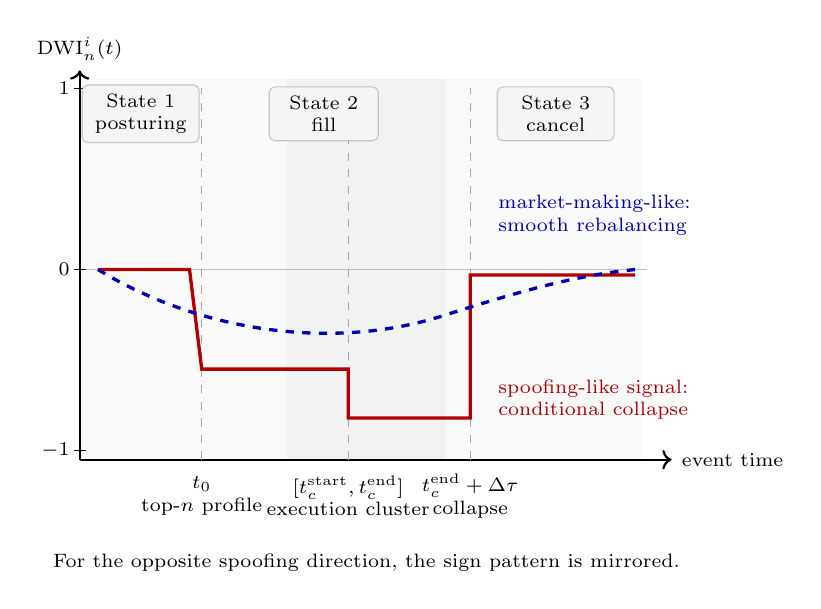
\begin{tikzpicture}[
        x=1.55cm,
        y=2.3cm,
        font=\scriptsize,
        axis/.style={->, thick},
        spoof/.style={very thick, red!70!black},
        maker/.style={very thick, dashed, blue!70!black},
        event/.style={gray!70, dashed},
        state/.style={fill=gray!8, draw=gray!45, rounded corners=2pt, align=center}
    ]
        \fill[gray!5] (0,-1.05) rectangle (1.7,1.05);
        \fill[gray!10] (1.7,-1.05) rectangle (3.0,1.05);
        \fill[gray!5] (3.0,-1.05) rectangle (4.6,1.05);

        \draw[axis] (0,-1.05) -- (0,1.1) node[above] {$\operatorname{DWI}_{n}^{i}(t)$};
        \draw[axis] (0,-1.05) -- (4.85,-1.05) node[right] {event time};
        \draw[gray!50] (-0.05,0) -- (4.65,0);

        \foreach \y/\lab in {-1/$-1$,0/$0$,1/$1$} {
            \draw (-0.05,\y) -- (0.05,\y) node[left=0.08cm] {\lab};
        }

        \draw[event] (1.0,-1.05) -- (1.0,1.0);
        \draw[event] (2.2,-1.05) -- (2.2,1.0);
        \draw[event] (3.2,-1.05) -- (3.2,1.0);

        \node[state, text width=1.25cm] at (0.5,0.86) {State 1\\posturing};
        \node[state, text width=1.15cm] at (2.0,0.86) {State 2\\fill};
        \node[state, text width=1.25cm] at (3.9,0.86) {State 3\\cancel};

        \node[align=center] at (1.0,-1.25) {$t_0$\\top-$n$ profile};
        \node[align=center] at (2.2,-1.25) {$[t_c^{\mathrm{start}},t_c^{\mathrm{end}}]$\\execution cluster};
        \node[align=center] at (3.2,-1.25) {$t_c^{\mathrm{end}}+\Delta\tau$\\collapse};

        \draw[spoof] (0.15,0) -- (0.9,0)
            -- (1.0,-0.55) -- (2.2,-0.55)
            -- (2.2,-0.82) -- (3.2,-0.82)
            -- (3.2,-0.03) -- (4.55,-0.03);

        \draw[maker] (0.15,0) .. controls (1.0,-0.35) and (2.1,-0.45) .. (3.0,-0.25)
            .. controls (3.7,-0.10) and (4.1,-0.03) .. (4.55,0);

        \node[red!70!black, align=left, anchor=west] at (3.35,-0.72) {spoofing-like signal:\\conditional collapse};
        \node[blue!70!black, align=left, anchor=west] at (3.35,0.30) {market-making-like:\\smooth rebalancing};
        \node[align=center] at (2.35,-1.62) {For the opposite spoofing direction, the sign pattern is mirrored.};
    \end{tikzpicture}
    \caption{Stylized cluster-time behavior of the multilevel distance-weighted imbalance. In the spoofing-compatible
    pattern, a large top-$n$ imbalance returns rapidly toward zero after the smaller opposite-side execution because the
    candidate profile is cancelled. The illustrative market-making path shows smoother inventory rebalancing.}
    \label{fig:topn_imbalance_dynamics}
\end{figure}
\FloatBarrier

\subsubsection{Conditional Withdrawal Reconstruction}
\label{subsec:multilevel_conditionality}

A static multilevel imbalance cannot establish manipulative intent. A market maker can also become temporarily imbalanced
while controlling inventory or responding to adverse selection. The additional observable feature is whether the profile
disappears conditionally after the participant's execution on the opposite side, as predicted by the stylized mechanism.

Let $c$ denote an execution cluster for participant $i$. Its ordered child fills share a passive order identifier, side,
price, and trading partition and satisfy the operational inter-fill-gap rule. The timestamps
$t_c^{\mathrm{start}}$ and $t_c^{\mathrm{end}}$ denote the first and last child fills. The quantity $Q_c$ is their total
executed quantity, and $s_c\in\{b,a\}$ is the passive execution side. We denote the opposite candidate-posture side by
$\bar{s}_c$. The pre- and post-cluster observation times are
\begin{equation}
    t_c^{-}=t_c^{\mathrm{start}}-\epsilon_t,
    \qquad
    t_c^{+}=t_c^{\mathrm{end}}+\Delta\tau,
\end{equation}
where $\epsilon_t$ places $t_c^{-}$ immediately before the first child fill and $\Delta\tau$ bounds the withdrawal window
after the final child fill.

We also impose a pre-execution episode window $\Theta>0$. An opposite-side order enters the candidate profile for cluster
$c$ only when its first observed posting time $\tau_o$ satisfies
\begin{equation}
    0 \leq t_c^{\mathrm{start}}-\tau_o \leq \Theta .
    \label{eq:deceptive_age_window}
\end{equation}
The empirical analysis uses $\Theta=90$ seconds as an exploratory default. Episode attribution therefore includes only
same-client top-$n$ orders first observed inside this pre-execution window. This restriction separates a recent candidate
layer from the participant's standing background liquidity. Without it, a nearly balanced long-lived profile could dilute
the measured withdrawal of a short-lived recent layer. We retain the unrestricted top-$n$ state to describe the
ordinary book footprint and use an \textit{episode-conditioned} profile for surveillance attribution.

Let $\mathcal{A}^{i,s}_{c,k,\Theta}(t)$ contain the active orders of client $i$ on side $s$ and rank $k\leq n$ at time
$t$ whose first observed posting time lies in
$[t_c^{\mathrm{start}}-\Theta,t_c^{\mathrm{start}}]$. Their episode-conditioned weighted liquidity is
\begin{equation}
    L^{i,s}_{c,n,\Theta}(t)
    =
    \sum_{k=1}^{n}
    \omega^{s}_{k}(t)
    \sum_{o\in\mathcal{A}^{i,s}_{c,k,\Theta}(t)}
    \widetilde q_o(t),
    \label{eq:episode_conditioned_liquidity}
\end{equation}
where $\widetilde q_o(t)$ is the visible quantity of order $o$, optionally normalized by the corresponding market depth as
in \cref{eq:relative_agent_depth}. We define the episode-conditioned imbalance as
\begin{equation}
    \operatorname{DWI}^{i}_{c,n,\Theta}(t)
    =
    \frac{
        L^{i,a}_{c,n,\Theta}(t)-L^{i,b}_{c,n,\Theta}(t)
    }{
        L^{i,a}_{c,n,\Theta}(t)+L^{i,b}_{c,n,\Theta}(t)+\varepsilon
    }.
    \label{eq:episode_conditioned_dwi}
\end{equation}
where the reported implementation fixes the numerical stabilizer at $\varepsilon=10^{-12}$. This statistic describes the
recent liquidity layer associated with cluster $c$, rather than the client's entire standing book. All subsequent collapse
and withdrawal diagnostics use this episode-conditioned profile.

The \textit{Spoofing Conditionality Index} measures the absolute change in its normalized shape:
\begin{equation}
    \operatorname{SCI}^{i}_{c,n}
    =
    \left|
        \operatorname{DWI}^{i}_{c,n,\Theta}(t_c^{-})
        -
        \operatorname{DWI}^{i}_{c,n,\Theta}(t_c^{+})
    \right|.
    \label{eq:topn_sci}
\end{equation}
An absolute imbalance change does not identify which side lost liquidity. We therefore also measure the fraction of
weighted liquidity that disappears from each side after the fill:
\begin{equation}
    C^{i,s}_{c,n}
    =
    \frac{
        \left[
            L^{i,s}_{c,n,\Theta}(t_c^{-})-L^{i,s}_{c,n,\Theta}(t_c^{+})
        \right]_{+}
    }{
        L^{i,s}_{c,n,\Theta}(t_c^{-})+\varepsilon
    },
    \qquad s\in\{b,a\},
    \label{eq:side_collapse}
\end{equation}
where $[x]_{+}=\max\{x,0\}$. A large $C^{i,\bar{s}_c}_{c,n}$ indicates that recent liquidity disappeared from the side
opposite to the clustered execution, as required by the mechanical sequence. A two-sided quote refresh after a mid-price
change can instead generate material collapse on both sides.

For a bounded event-level summary of these shape diagnostics, define the clipping operator by
\begin{equation}
    \operatorname{clip}_{[0,1]}(x)=\min\{\max\{x,0\},1\}.
\end{equation}
Then define
\begin{equation}
\begin{aligned}
    \widetilde{\operatorname{SCI}}^{i}_{c,n}
    &=\operatorname{clip}_{[0,1]}\!\left(\frac{1}{2}\operatorname{SCI}^{i}_{c,n}\right),\\
    \widetilde C^{i,s}_{c,n}
    &=\operatorname{clip}_{[0,1]}\!\left(C^{i,s}_{c,n}\right),\\
    \operatorname{MSCI}^{i}_{c,n}
    &=\frac{1}{3}\left[
        \widetilde{\operatorname{SCI}}^{i}_{c,n}
        +\widetilde C^{i,\bar{s}_c}_{c,n}
        +\left[\widetilde C^{i,\bar{s}_c}_{c,n}-\widetilde C^{i,s_c}_{c,n}\right]_{+}
    \right].
\end{aligned}
    \label{eq:additive_msci}
\end{equation}
Because DWI lies in $[-1,1]$, the normalized shape term and both collapse terms lie in $[0,1]$, so MSCI also lies in
$[0,1]$. The arithmetic mean gives equal weight to shape change, opposite-side withdrawal, and side asymmetry without
allowing a zero in one component to erase the remaining diagnostics. The components remain separately inspectable so that
a two-sided quote refresh is distinguishable from an asymmetric collapse. MSCI is retained as a secondary event-level
diagnostic and in client-level feature summaries; it does not enter the four-condition event gate or the generated result
tables.

\subsubsection{Canonical Matched Withdrawal}
\label{subsec:canonical_matched_withdrawal}

A cancellation can be eligible for several nearby execution clusters. To measure withdrawal without counting that
cancellation more than once, let $\mathcal E(o)$ contain the eligible same-client, opposite-side clusters that precede
cancellation $o$ by at most $\Delta\tau$. We assign $o$ deterministically to the canonical cluster
\begin{equation}
    a(o)=\underset{c\in\mathcal E(o)}{\arg\min}\,
    \left(t_o-t_c^{\mathrm{end}},\;t_c^{\mathrm{start}},\;\operatorname{id}_c\right),
    \label{eq:canonical_cancel_assignment}
\end{equation}
where the tuple is ordered lexicographically and the stable cluster identifier breaks any final tie. Eligibility also
requires source-sequence precedence: the cancellation follows the cluster's final child fill in both event time and source
sequence. For eligible top-$n$ cancellations, define $\mathcal{C}_{c,n}^{i}=\{o:a(o)=c\}$. A physical cancellation is
identified by its trading partition, source index, and candidate order identifier. We preserve every eligible link for
audit, but each physical cancellation contributes to at most one cluster's metrics.

For each assigned order $o\in\mathcal{C}_{c,n}^{i}$, let $q_o$ denote its visible quantity immediately before
cancellation. The total assigned withdrawal and its ratio to cluster quantity are
\begin{equation}
    U^{i}_{c,n}=\sum_{o\in\mathcal{C}_{c,n}^{i}}q_o,
    \qquad
    R^{i}_{c,n}=\frac{U^{i}_{c,n}}{Q_c+\varepsilon},
    \label{eq:assigned_withdrawal}
\end{equation}
where $Q_c$ is the execution-cluster quantity. Let $Q^{i,\bar{s}_c}_{c,n}$ denote the visible quantity of the candidate
profile before execution. We report the fraction of that profile removed as
\begin{equation}
    A^{i}_{c,n}
    =\frac{U^{i}_{c,n}}{Q^{i,\bar{s}_c}_{c,n}+\varepsilon}.
    \label{eq:assigned_withdrawal_share}
\end{equation}
These quantities remain separately inspectable. The full descriptive gate requires $U^{i}_{c,n}>Q_c$ rather than applying
a threshold to a composite score. We summarize repeated behavior through counts and withdrawal rates at the
client--partition level. We do not use a scalar aggregate to rank clients or infer intent.

\subsubsection{Price-Response Diagnostics}
\label{subsec:price_response_diagnostics}

The matched-withdrawal variables show whether a client removes same-client opposite-side liquidity after its own
execution. They do not show whether the price path is consistent with the hypothesized mechanism. Such a path first moves
in the direction favorable to the clustered execution and then partly reverses after the candidate layer is removed. We
measure these two features with separate price-response diagnostics. They are economic consistency checks, not causal
estimates of manipulation.

Let $b(t)$ and $a(t)$ denote the best bid and ask, with corresponding displayed quantities $q^b_1(t)$ and $q^a_1(t)$. When
both quotes and positive top-level depth are available, the two market-price proxies are the mid-price
$M_{\mathrm{mid}}(t)=[a(t)+b(t)]/2$ and the queue microprice
$M_{\mathrm{micro}}(t)=[a(t)q^b_1(t)+b(t)q^a_1(t)]/[q^b_1(t)+q^a_1(t)]$
\cite{Stoikov02122018}; otherwise the corresponding diagnostic is missing. Let $M(t)$ denote either proxy, and let $t_0$
be the earliest first-observed posting time among the eligible candidate orders for cluster $c$. We encode the clustered
execution direction as
\begin{equation}
    h_c=
    \begin{cases}
        +1, & \text{if the clustered passive execution is a sell execution,}\\
        -1, & \text{if the clustered passive execution is a buy execution.}
    \end{cases}
    \label{eq:price_response_direction}
\end{equation}
Under this convention, a positive signed change is favorable to the execution: a sell benefits from an upward move and a
buy from a downward move. We measure the favorable movement between candidate-layer posting and execution as
\begin{equation}
    \operatorname{FPM}^{i}_{c}
    =
    h_c\left[M(t_c^{-})-M(t_0)\right],
    \label{eq:favorable_price_move}
\end{equation}
Reversion is anchored to each assigned cancellation rather than to the end of the execution cluster. Let $t_o$ denote the
cancellation timestamp, $t_o^{-}$ the last reconstructed state strictly before its source index, and $H_R=2$ seconds the
reversion horizon. Let $\mathcal{C}_{c,n}^{i,\mathrm{obs}}$ contain the assigned cancellations with both pre-cancellation
and horizon states. The cluster-level post-cancellation reversion is the quantity-and-delay weighted mean
\begin{equation}
    \operatorname{REV}^{i}_{c}
    =
    \frac{
        \sum_{o\in\mathcal{C}_{c,n}^{i,\mathrm{obs}}}
        w_{c,o}h_c\left[M(t_o^{-})-M(t_o+H_R)\right]
    }{
        \sum_{o\in\mathcal{C}_{c,n}^{i,\mathrm{obs}}} w_{c,o}
    },
    \qquad
    w_{c,o}=q_o\exp\!\left(-\frac{t_o-t_c^{\mathrm{end}}}{\tau_w}\right),
    \label{eq:price_reversion}
\end{equation}
with $\tau_w=10$ seconds in the reported run. Here $M(t_o+H_R)$ denotes the last reconstructed state at or before the
target time, provided that the message sequence covers that target. The statistic is missing when no assigned cancellation
has an observable horizon state.
A positive $\operatorname{FPM}^{i}_{c}$ means that the price moved in the direction favorable to the clustered execution
while the candidate layer was present. A positive $\operatorname{REV}^{i}_{c}$ means that the market-price proxy moved
against the pre-fill favorable direction after the assigned cancellation or cancellations. For quantity-weighted cluster
price $P_c$, we also define the local execution advantage relative to the pre-posture benchmark:
\begin{equation}
    \operatorname{ADV}^{i}_{c}
    =
    h_c\left[P_c-M(t_0)\right].
    \label{eq:execution_advantage}
\end{equation}
The execution advantage is positive when a sell executes above the benchmark or a buy executes below it.

We compute each diagnostic with both the mid-price and the queue microprice in the event-level artifacts. The generated
summary tables and the event gate use the mid-price versions. We report price responses separately from withdrawal counts,
quantities, and rates instead of multiplying all components into one detector. Withdrawal variables describe the
reconstructed message sequence. The variables $\operatorname{FPM}$, $\operatorname{REV}$, and $\operatorname{ADV}$
describe the associated price path. This separation distinguishes repeated conditional withdrawals without a favorable
price response from episodes that also exhibit favorable pre-fill movement and post-cancellation reversion.

\subsubsection{Event Reconstruction}
\label{subsec:event_reconstruction}

We reconstruct events from order-level messages rather than aggregate snapshots. A resting order can change book rank
when the best quote moves even though its owner has neither modified nor cancelled it. Snapshot changes alone can therefore
confound repricing of the surrounding book with withdrawal by the participant. The operational procedure is:
\begin{enumerate}
    \item Identify compatible passive child fills and construct cluster $c$, preserving the ordered mapping to raw messages.
    \item Reconstruct participant $i$'s active orders immediately before $t_c^{\mathrm{start}}$.
    \item Assign each active order to side $s$ and rank $k\leq n$. Retain in the episode-conditioned profile
    only orders whose first observed posting time lies in
    $[t_c^{\mathrm{start}}-\Theta,t_c^{\mathrm{start}}]$.
    \item Compute $L^{i,b}_{c,n,\Theta}(t_c^{-})$, $L^{i,a}_{c,n,\Theta}(t_c^{-})$, and
    $\operatorname{DWI}^{i}_{c,n,\Theta}(t_c^{-})$.
    \item Apply executions, cancellations, and amendments through
    $[t_c^{\mathrm{start}},t_c^{\mathrm{end}}+\Delta\tau]$.
    \item Retain every eligible cluster--cancellation link. Assign each physical cancellation canonically using
    \cref{eq:canonical_cancel_assignment}, and exclude competing links from metric totals.
    \item Compute the corresponding episode-conditioned quantities at $t_c^{+}$.
    \item Report assigned withdrawal quantity, withdrawal-to-fill ratio, and removed-profile fraction.
    \item Compute signed price diagnostics from the first candidate-layer posting, through the cluster, to the
    post-cancellation window.
    \item Summarize repeated behavior with cluster counts and client-level recurrence diagnostics. Retain raw child-fill
    messages as provenance.
\end{enumerate}
This procedure is designed to distinguish ordinary book repricing from withdrawal of participant-attributed candidate
liquidity. Canonical assignment ensures that one physical cancellation does not inflate the metrics of several neighboring
clusters under the stated eligibility rule.

The event-level \textit{spoofing-compatible sequence} gate requires four observed conditions: a rapid assigned
withdrawal, withdrawn quantity greater than cluster fill quantity, positive favorable pre-fill mid-price movement, and
positive mid-price reversion from the assigned cancellation over an observable $2$-second horizon. Right-censored
reversion outcomes fail the gate. This transparent conjunction supports analyst triage; it is descriptive and is not a
statistical test, manipulation label, or proof of intent.

The all-sample run uses a $10$-second structural window, $2$-second rapid-attribution and cancel-anchored reversion
windows, and a $90$-second candidate-order age limit. We estimate the empirical top-$10$ kernel separately for each
instrument. The reported outputs keep withdrawal and price-response components separate rather than reducing them to a
scalar composite score.

\section{Results}
\label{sec:results}

\subsection{Cross-Instrument Detection Summary}
\label{subsec:cross_instrument_results}

We apply the same episode-conditioned top-$10$ reconstruction to all three samples.
\Cref{tab:empirical_spoofing_diagnostics} reports the resulting exploratory diagnostics. Each instrument uses its
full-sample empirical kernel from \cref{tab:empirical_depth_kernel_calibration} with $H=10$ seconds.

A matched cluster is an aggregated passive execution followed within $2$ seconds by a canonically assigned, same-client
cancellation of an opposite-side candidate order. The separate $10$-second interval is the structural reconstruction
horizon. The table distinguishes execution clusters from their raw child fills and counts each assigned physical
cancellation once. The price-response columns report the share of matched clusters with positive signed mid-price
favorable movement ($\operatorname{FPM}>0$) and the share with positive post-cancellation reversion
($\operatorname{REV}>0$). These quantities are descriptive screening diagnostics, not manipulation labels or evidence of
intent.

\InputIfFileExists{generated/spoofing_empirical_tables.tex}{}{%
    \fbox{\parbox{0.9\textwidth}{Run \texttt{scripts/generate\_spoofing\_paper\_tables.py} to generate the empirical tables.}}%
}

The reported empirical quantities are direct reconstruction counts and conditional descriptive shares. No counterfactual
comparison or inferential test is applied, so the table does not provide $p$-values, confidence intervals, or evidence that
withdrawal is more likely after the focal client's own fill than under an otherwise comparable no-fill condition.

\subsection{Risanamento}
\label{subsec:risanamento_results}

The Risanamento sample contains \RisanamentoRawFills{} raw passive child fills, which the clustering rule consolidates into
\RisanamentoClusters{} execution clusters. Canonical linkage identifies \RisanamentoMatchedClusters{} clusters followed by
at least one assigned, same-client, opposite-side withdrawal. These clusters own
\RisanamentoAssignedCancellations{} physical cancellations in total. A cluster can own several cancellations, but each
cancellation is assigned to at most one cluster. Among rapid matched clusters, \RisanamentoFPMShare{} have positive
favorable pre-fill mid-price movement and \RisanamentoREVShare{} have positive cancel-anchored reversion.

The event-review dashboard contains a cluster-first dossier and reconstructed top-$10$ window for each of the
\RisanamentoMatchedClusters{} matched clusters. These review objects organize observed facts, counter-evidence, and
legitimate alternatives. They are triage aids, not empirical labels or proof of manipulation.

\subsection{Nexi}
\label{subsec:nexi_results}

The Nexi sample contains \NexiRawFills{} raw passive fills and \NexiClusters{} execution clusters. Reconstruction identifies
\NexiMatchedClusters{} matched clusters and \NexiAssignedCancellations{} canonically assigned physical cancellations.
Positive favorable pre-fill movement occurs in \NexiFPMShare{} of matched clusters, and positive cancel-anchored reversion
occurs in \NexiREVShare{}.

Differences from the other instruments are not causal contrasts because the samples cover different periods and client
compositions.

\subsection{Ferrari}
\label{subsec:ferrari_results}

The Ferrari sample contains \FerrariRawFills{} raw passive fills and \FerrariClusters{} execution clusters. Reconstruction
identifies \FerrariMatchedClusters{} matched clusters and \FerrariAssignedCancellations{} canonically assigned physical
cancellations. The shares with positive favorable pre-fill movement and positive reversion are \FerrariFPMShare{} and
\FerrariREVShare{}.

These are descriptive screening outcomes, not manipulation labels or prevalence estimates.

\subsection{Client-Level Attribution and Interpretation}
\label{subsec:client_level_results}

\Cref{tab:top_client_results} ranks attributable client groups by matched-cluster count. Its W/F maximum is the
largest matched withdrawal-to-fill ratio within the group; FPM$+$ and REV$+$ are the shares of matched clusters with
positive mid-price favorable movement and reversion. The table omits unknown or missing identifiers from these rankings.
The accompanying CSV reports their cluster counts separately. This rule prevents a placeholder such as ``0'' from being
interpreted as a verified economic actor.

The primary empirical object is the participant-level association between execution and rapid opposite-side withdrawal.
We report its magnitude and repetition descriptively. An analyst must also consider the withdrawn order's execution risk
and distance from the touch, bilateral activity, inventory context, price response, and execution advantage. Together,
these diagnostics indicate whether an episode is economically consistent with the stylized mechanism or remains compatible
with legitimate liquidity provision. Neither a scalar score nor a dashboard review category is treated as ground truth.

\section{Discussion and Conclusion}
\label{sec:discussion_conclusion}

Across these three samples, the reconstruction identifies rapid same-client withdrawal episodes and associated price paths.
These outcomes describe the stated reconstruction and thresholds; they neither estimate spoofing prevalence nor establish
that any retained sequence was manipulative.

Several limitations constrain interpretation. The depth kernels are calibrated on the same full samples to which they are
applied, so their displayed-price associations are descriptive rather than out-of-sample evidence. The analysis does not
include a counterfactual statistical test, and repeated events from the same clients or trading periods need not be
independent. Right-censored reversion outcomes fail the event gate, and the reported results do not test sensitivity to the
$100$-millisecond child-fill clustering threshold. The three instrument samples also cover different periods and client
compositions, which rules out causal cross-instrument comparisons.

The contribution is therefore an auditable surveillance workflow rather than an enforcement classifier. It preserves raw
message provenance, separates withdrawal from price-response evidence, and exposes the gate conditions used for triage.
Prospective use would require a pre-specified counterfactual design and thresholds, kernel calibration on training periods
only, chronological out-of-sample validation, and evaluation against independently reviewed cases with explicit
false-positive and false-negative costs.

% We propose two agent-specific metrics based on the
% microprice and the volume-distance correlation. 
% \paragraph{Agent-Specific Microprice ($m_i$)} The traditional microprice is widely 
% recognized in high-frequency trading as a robust estimator of the expected future mid-price \cite{Stoikov02122018}, uniquely synthesizing both 
% the price and volume dimensions of the limit order book. By isolating this calculation to a single participant's resting 
% orders, we can formulate an an agent-specific microprice ($m_i$) to quantify its personal vision of the future price::

% \begin{equation}
%     m_i = \frac{a_iV^b_i + b_i V^a_i}{V^b_i + V^a_i} = \frac{a_i + b_i}{2} + \frac{a_i-b_i}{2} \frac{V_i^b-V_i^a}{V_i^b+V_i^a} = \text{mid-price} + \frac{\text{spread}}{2} \times \text{imbalance}
% \end{equation}
% Where $a_i$ and $b_i$ represent the agent's ask and bid prices, and $V^a_i$ and $V^b_i$ represent their respective 
% volumes. Legitimate market makers, constrained by inventory risk, typically maintain symmetric quotes ($V^b_i \approx V^a_i$) 
% to capture the spread, resulting in an $m_i$ that closely tracks the fundamental mid-price. Conversely, a spoofer 
% deliberately engineers an extreme unbalanced environment to manipulate the heuristics of victim algorithms. 
% Consequently, a spoofer's $m_i$ will drastically diverge from the true mid-price.

% \paragraph{Correlation Between Posting Distance ($\delta$) and Volume} The second metric mathematically formalizes the 
% spoofer's optimization dilemma by measuring the correlation between an agent's order volume and their posting distance 
% ($\delta$) from the best bid or ask. Empirical models confirm that posting distance is a critical determinant of price 
% impact, and its omission renders LOB detection models mathematically inadequate.Because market makers seek execution to 
% earn the bid-ask spread, their inventory management necessitates posting their largest order volumes at or adjacent to 
% the top of the book ($\delta \approx 0$). Spoofers, conversely, optimize a strictly directional expected cost function: 
% they must maximize the psychological and algorithmic impact of their non-bona fide volume while minimizing the risk of 
% inadvertent execution. This is achieved by placing a small, bona fide order at a minimal distance ($\delta \approx 0$) 
% to guarantee execution, and a massive, non-bona fide order at a significantly larger distance deeper within the opposite 
% side of the LOB ($\delta \gg 0$) to act as a structural buffer against aggressive market orders. Thus, observing a strong 
% correlation between massive volume and a large $\delta$ on one side of the book—paired with small volume and a minimal 
% $\delta$ on the execution side—serves as and additional microstructural signature of a manipulative strategy.


\bibliographystyle{abbrv}
\bibliography{references}

\end{document}
